\documentclass[aagreenthesis]{subfiles}
%\usepackage{macros}
%\externaldocument[I-]{chap1}
\begin{document}
\chapter{The Discovery of Helicity in Tilted Bent-Core Smectics: \smcpalpha{}}
\todo{put joe prc in beginning of subsection}
\todo{put biref/tilt figure in the optical textures/electro-optics section}

The discovery of spontaneous macroscopic polar
ordering~\cite{niori_distinct_1996} and chirality~\cite{link_spontaneous_1997} in
fluid smectic liquid crystal phases of achiral  bent-core mesogens has led to
the exploration of a rich family of novel liquid crystal phases and
self-assemblies~\cite{takezoe_bent-core_2006,eremin_polar_2013,takezoe2017bent,chattham_triclinic_2010,reddy_spontaneous_2011}
 in which the key macroscopic elements of polarity, chirality, and smectic layering all appear as spontaneously broken symmetries.
While the smectic layer-scale order of bent-core mesogens, resulting from strong intralayer
coupling between molecular tilt and polarity, is quite well characterized, superlayer
structuring beyond that of the four basic SmCP bilayer phases combining synclinic or
anticlinic tilt with ferroelectric or antiferroelectric
polarity~\cite{link_spontaneous_1997}, as sketched in Supplemental Figure~S1, have
not been definitively identified.
Possible superlayer structures analogous to those seen in tilted SmC*
phases of chiral, rod-shaped molecules could be incommensurate or commensurate with the
underlying smectic layer spacing and feature states of varying azimuthal orientation
of the molecular long axis about the layer normal, $z$, such as the chiral
helical precession along $z$ with equal, discrete orientational jumps between layers of
the $\mathrm{SmC}^*_\alpha$ phase and the ferrielectric phases with periodic arrays of discrete jumps of
different sizes~\cite{takezoe2010antiferroelectric}.

Since the period of such superlayer structures, $p$,  can be as short as two
layers, the structural study of such phases requires the
effective probing of molecular orientation at the nanoscale. This can be
achieved using resonant X-ray scattering, a technique sensitive to atomic
environment~\cite{mach_structural_1998,levelut1999tensorial,mach_structures_1999,hirst2002interlayer,gleeson_resonant_2006,Barois2012review,folcia2014spontaneous,huang2015liquid,zhu2015probing,zhu2016resonant,salamonczyk2017structure}
that has previously enabled the discovery and
definitive characterization of superlayer organization in several SmC* phases and sub-phases, employing
the K-edge resonance of atoms incorporated in the liquid crystal molecule~\cite{mach_structural_1998,mach_structures_1999}.

Several recent
observations suggest the possibility of chiral superlayer ordering in achiral
bent-core mesogens: Takanishi et al.\ have identified such a structure in a
SmCP phase of a bent-core mesogen doped with a chiral, rod-shaped molecule that as a neat
material exhibits $\mathrm{SmC}^*_\alpha$ and ferrielectric phases~\cite{takanishi2015chiral};
Abberley et al.\ have reported a superlayer helix in a smectic phase of bent dimers of molecular
rods~\cite{abberley2018heliconical}; Panarin and co-workers have recently proposed,
based on AFM
evidence, the existence of tilted, helical supermolecular ordering in several achiral bent-core mesogens with $4$-cyanoresorcinol bisbenzoate cores~\cite{sreenilayam_spontaneous_2016}.
Earlier investigations of this molecular family had concluded, however, that their polar phases were orthogonal, i.e.,  untilted and therefore not chiral~\cite{panarin_sequence_2011,sreenilayam_properties_2012}.
Motivated by these conflicting reports and the ongoing interest in the chiral sub-phases of liquid crystals, we have studied one of the members of this
homologous series, \nfour{phi}, which has $n = 14$ alkyl tails (see Figure~\ref{fig:main}(a)). Our experiments, using
non-resonant X-ray scattering (SAXS), resonant soft X-ray scattering (RSoXS), electro-optic techniques, and polarized light
microscopy (PLM), summarized in Figure~\ref{fig:main}, reveal an exotic phase sequence, including
an achiral de Vries smectic which becomes chiral in sufficiently large applied
electric fields, and, at lower temperature, a tilted, chiral smectic with superlayer helical
ordering.
\section{Characterization of \nfour{}}
We used a combination of two-dimensional, small-angle, hard X-ray scattering
(SAXS),  resonant, soft X-ray scattering (RSoXS), differential scanning
caliorimetry (DSC), polarized, transmitted light microscopy on cells in
transmission, and measurements of the polarization reversal current of cells in
order to characterize \nfour{phi}. These experiments reveal four smectic
phases, labeled in order of descending temperature as Sm1, Sm2, Sm3, and Sm4.


\subsection{Experimental Details}
The RSoXS experiments were performed at the Advanced Light Source at Lawrence
Berkeley National Laboratory beamline 11.0.1.2 using linearly polarized X-ray
photons~\cite{wang2011defining, liu2016resonant}. The X-ray energy was tuned
between \SI{270}{\eV} and \SI{290}{\electronvolt} in our experiments, with
scattering contrast appearing only for energies near the carbon K-edge resonance (E =
\SI{284}{\electronvolt}), indicating the presence of real-space features with an orientational modulation.
The \nfour{phi} material was sandwiched between two silicon nitride substrates,
while in the isotropic phase. The cell was then placed into a temperature
controlled hotstage in the beamline.
After finding the highest temperature where scattering features were observed,
the sample was cooled slowly while recording $2$D diffractograms of the scattering. The
RSoXS setup is sensitive to orientational modulations from $d=$ \SIrange{50}{1250}{\angstrom}. The relative positions and orientations of the sample and detector were calibrated using a
sample with known scattering $q$-values. The data from the detector was processed using the
Igor Pro-based NIKA data reduction software package~ \cite{ilavsky2012nika, zhang2010glassy}.

The angular resolution of the diffractometer, estimated from the full width at
half-maximum of a resonant feature known to be twice the smectic layer spacing
is $\delta q \sim \SI{.00078}{\angstrom^{-1}}$.

SAXS measurements were carried out on beamline X10A of the National Synchrotron
Light Source (NSLS), at Brookhaven National Laboratory. This beamline has a Si 111 double monochromator, tuned to around \SI{10}{\kilo\electronvolt}. The sample was mounted in an Instec hot stage on a Huber four-circle goniometer.
%
The angular resolution of the diffractometer, measured by scanning the detector arm
through the attenuated direct beam, is $\delta q \sim
\SI{0.005}{\nano\metre^{-1}}$ full width at half-maximum.

The planar cells used for texture analysis were \SI{4.5}{\micro\metre} thick commercial cells purchased from Instec Inc.\ with rubbed polyimide planar alignment layers and ITO glass. The thickness of the empty cells was measured using a visible light spectrometer. The cells were then filled with \nfour{phi} in the isotropic phase.  Polarization reversal current was measured in these cells by applying an alternating, triangular voltage.

The birefringence was measured using a Zeiss quartz-wedge compensator and a
\SI{5.86}{\micro\metre} thick Instec cell.

The molecular length of \nfour{phi} was estimated using a Hartree-Fock 6-31G*
calculation of a single molecule in the gas phase using the Spartan ‘16
numerical calculation package.


\begin{figure}
    \centering
    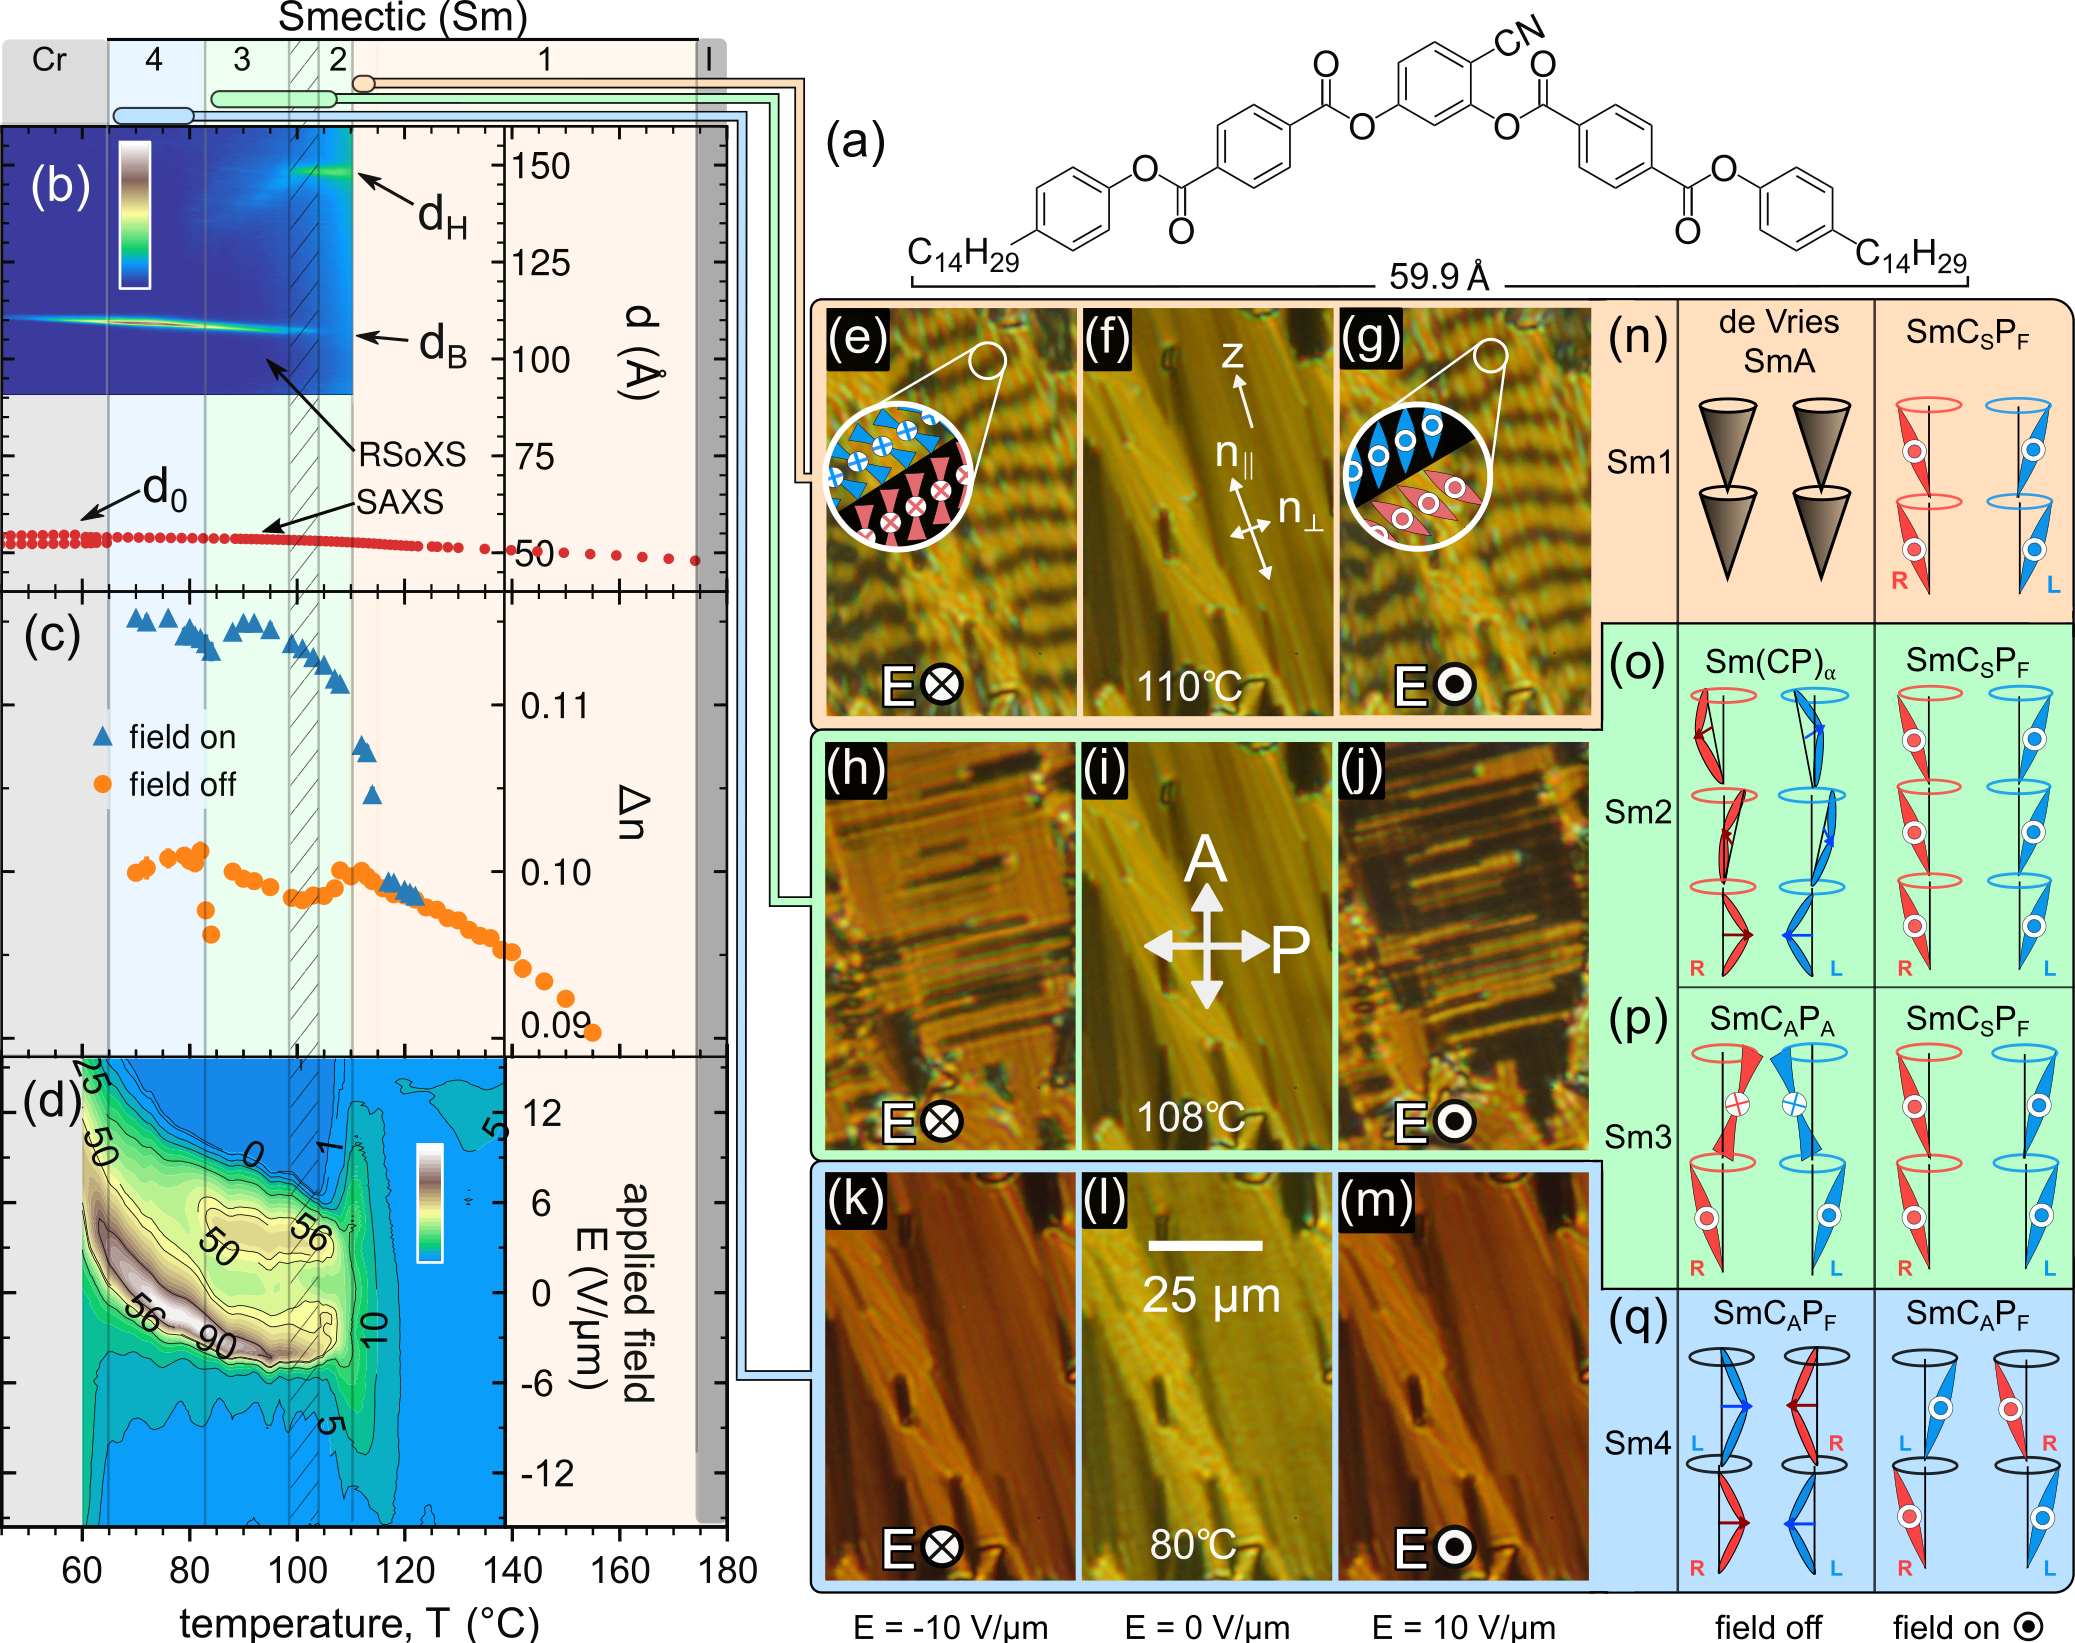
\includegraphics[width=.9\textwidth]{figs/pal30/fromPaper/finalFigs/Figure1v3.png}
    \caption{\label{fig:main}
        Experimental characterization of \nfour{phi}. (a) The \nfour{phi} molecule, showing the
        all-trans length calculated using the program Spartan. (b--d) Phase properties vs.\ temperature. The solid vertical lines denote phase boundaries and the cross-hatching phase coexistence.
    (b) SAXS shows the smectic layer spacing in all
    phases to be $d_0 \approx \SI{48}{\angstrom}$. Resonant carbon K-edge
    reflections are from superlayer
    modulations of the molecular orientation about the layer normal $z$, the peak
    at $d_H \approx \SI{150}{\angstrom}$ corresponding to the pitch of the incommensurate, helical precession in the Sm2 phase, and at
    $d_\text{B}=2d_0$ to the bilayer ordering of the Sm3 and Sm4 phases.
    (c) Birefringence of planar-aligned cells with layers normal to the plates, with and without applied electric
    field ($E = \SI{20}{\volt\per\micro\metre}$).
    (d) Polarization current (in nA) in response to a triangle-wave applied electric field:
    a single-peak, Langevin-like response at lower
    temperatures in the Sm1
    phase; a triple peak in the Sm2 phase, associated with ferrielectric
    switching\cite{findeisen2008multistage} and indicative of helical
    unwinding\cite{takezoe2010antiferroelectric}, coalescing into a double peak in the Sm3, indicating a
    non-polar ground state at $E = 0$; and a single current peak in the Sm4 phase
    caused by the block polarization switching of the ferroelectric \smcapf{phi} ground state.
    (e--m) Characteristic optical textures in a planar cell, viewed between
    crossed polarizers. The $E = 0$ textures are
    focal conics typical of a fluid smectic with an optic axis along $z$.
    Field application induces chiral, tilted conglomerate domains (of opposite
    handedness) in the Sm1--Sm3 phases, but only a
    change in birefringence in the Sm4.
    (n--q) Proposed superlayer structure of \nfour{phi} phases, with and without
    applied electric field: (n) Sm1: achiral de Vries-like SmA
    $\rightarrow$ chiral \smcspf{phi};  Sm2: superlayer chiral helix
    $\rightarrow$ chiral \smcspf{phi}; Sm3: superlayer chiral bilayer
    \smcapa{phi} $\rightarrow$ chiral \smcspf{phi}; Sm4: \smcapf{phi} with
    $\textbf{P}$ parallel to the glass $\rightarrow$ \smcapf{phi}
    with $\textbf{P}$ normal to the glass.
            }
\end{figure}

\subsection{Differential Scanning Caliorimetry of \nfour{}}

\begin{figure}[h!]
    \centering
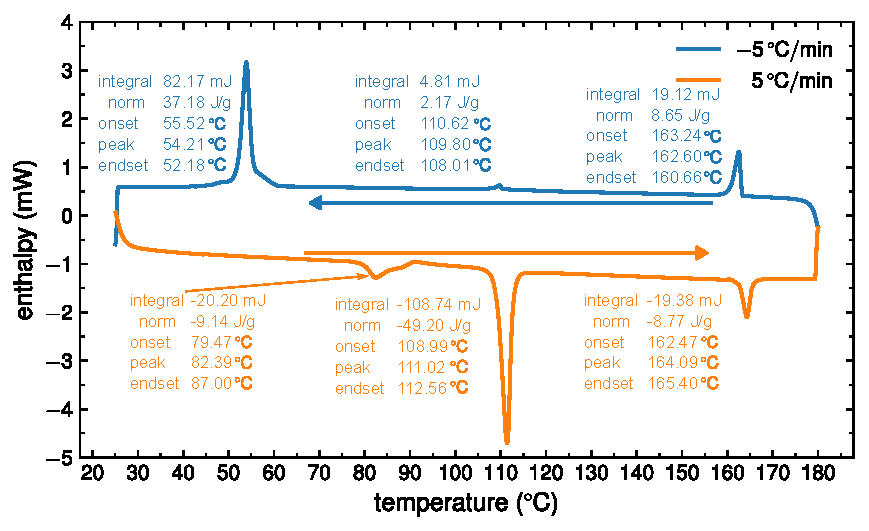
\includegraphics[width=\textwidth]{figs/pal30/fromPaper/figsForThesis/dsc/dsc-slowrun.pdf}
    \caption{\label{fig:pal30:dsc} Differential scanning caliorimetry of
        \nfour{}. On cooling, there is only a small, enthalpy peak at $\approx
    \SI{110}{\degreeCelsius}$ corresponding to the transition from the
highest-temperature smectic phase, the Sm1, and the Sm2.}
\end{figure}

The DSC reveals only a single enthalpy peak on cooling, at approximately
\SI{110}{\degreeCelsius}, hinting that the
Sm1~$\rightarrow$~Sm2 transition is either a weakly first order, or a second
order transition.


The lack of other enthalpy peaks is concerning, considering we identify four
unique smectic phases in the phase sequence of \nfour{}. However, the
resonant scattering experiments described in \autoref{sec:pal30:xray},
particulary the soft-melting mode seen in Figures~\ref{fig:pal30:diffractVt},
shows that the phase transition from the
Sm2~$\rightarrow$Sm3 is strongly second order, spanning a temperature range
of \SI{10}{\degreeCelsius}, which explains the absence of a distinct enthalpy peak in
the DSC for this transition 

The lack of a distinct peak for the Sm3~$\rightarrow$~Sm4 peak has two
plausible explanations. First, the polarization current shown in
\autoref{fig:pal30:prcbig} shows that the
transition is likely second order, spanning a temperature range of
approximately \SI{5}{\degreeCelsius}, like the
Sm2~$\rightarrow$~Sm3. Though, as the identified structures of the Sm3
(\smcapa{}) and Sm4 (\smcapf{})
cannot be connected by a continuous deformation the same way the helical Sm2
(\smcpalpha{}) can be deformed into the Sm2 (\smcapa{}), this seems less
likely. 

The other explanation, which I consider more likely, is due to the fact the DSC
is measured
without a field present, raising the possibility first explored by
Guzman\cite{edThesis} for orthogonal phases, that the transition from the \smcapa{} to the
\smcapf{} could be a kinetic trap. If this was the case, then the
\smcapa{} would be expected to be the ground-state phase \textit{in absence
of an applied field} for the remainder of
the phase sequence. This could be tested in future experiments with
the DC hysterises measurements described in Dr. Guzman's
thesis\cite{edThesis}.



\subsection{X-ray Scattering of \nfour{}}
\label{sec:pal30:xray}
X-ray scattering from \nfour{phi} is shown in Figures~\ref{fig:main}(b) and S3.

Upon  cooling from the isotropic, a single, non-resonant SAXS peak
appears at $\SI{175}{\degreeCelsius}$, at a wavevector $q_0$  corresponding to Bragg scattering from
the smectic layers in the Sm1 phase with spacing $d_0 = 2\pi/q_0
= \SI{48}{\angstrom}$. 


\begin{figure}[h!]
    \centering
    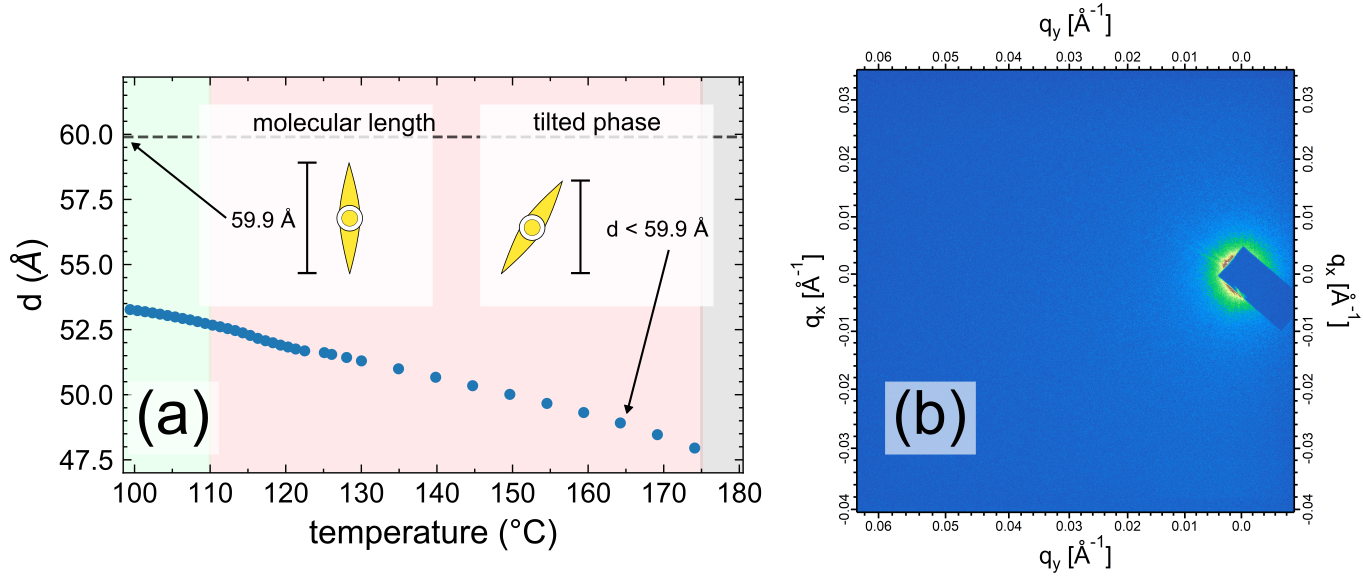
\includegraphics[width=\textwidth]{figs/pal30/xraysm1/sm1-xray-annote.png}
    \caption{\label{fig:pal30:saxs} X-ray scattering of high temperature phase,
        Sm1, of \smcpalpha{}. (a) The smectic layer
    size, $d$, increases monotonically on cooling, with no inflection points
that would be characteristic of a untilted$\rightarrow$tilted phase transition.
(b) No resonant scattering is observed for this phase.}
\end{figure}


The layer spacing increases slightly on cooling
to the crystal phase at \SI{65}{\degreeCelsius} and is
consistently smaller than the calculated molecular length, $l = \SI{59.9}{\angstrom}$, throughout this temperature range, suggesting that the molecules are tilted in all of the smectic phases, to first order by an average amount estimated using $\theta_\textrm{xray} =
\cos(d_0/l)$ of $\SI{33}{\degree}$ (see Figure~S4).
In the Sm1 temperature range ($\SI{110}{\degreeCelsius} \leq T \leq
\SI{175}{\degreeCelsius}$), there are no RSoXS scattering features
(\autoref{fig:pal30:saxs} (b) ) that would indicate a
superlayer periodic structure.

At the transition to the Sm2 phase, at $\SI{110}{\degreeCelsius}$, marked  by
a distinct enthalpy peak in the DSC (Figure~S5
), a single, sharp
resonant peak appears at $q_H = \SI[per-mode=reciprocal]{.042}{\per\angstrom}$, corresponding
to a molecular orientational structure with a period
$d_H=\SI{148}{\angstrom}\approx 2.8 d_0$ that is incommensurate with the
smectic layer spacing (Figure~\ref{fig:xray-results}(b) and
\autoref{fig:pal30:diffractVt}). Below
$\SI{104}{\degreeCelsius}$, this reflection
becomes weaker and another sharp, resonant reflection at higher $q$ grows in, the coexistence
indicating a first-order transition to the Sm3 phase.
This second Bragg peak, which persists down to the crystal phase, has a
wavevector $q_B\approx q_0/2$, indicative of a commensurate, bilayer orientational
structure in the Sm3 and Sm4 phases.
%

\begin{figure}[h!]
    \centering
    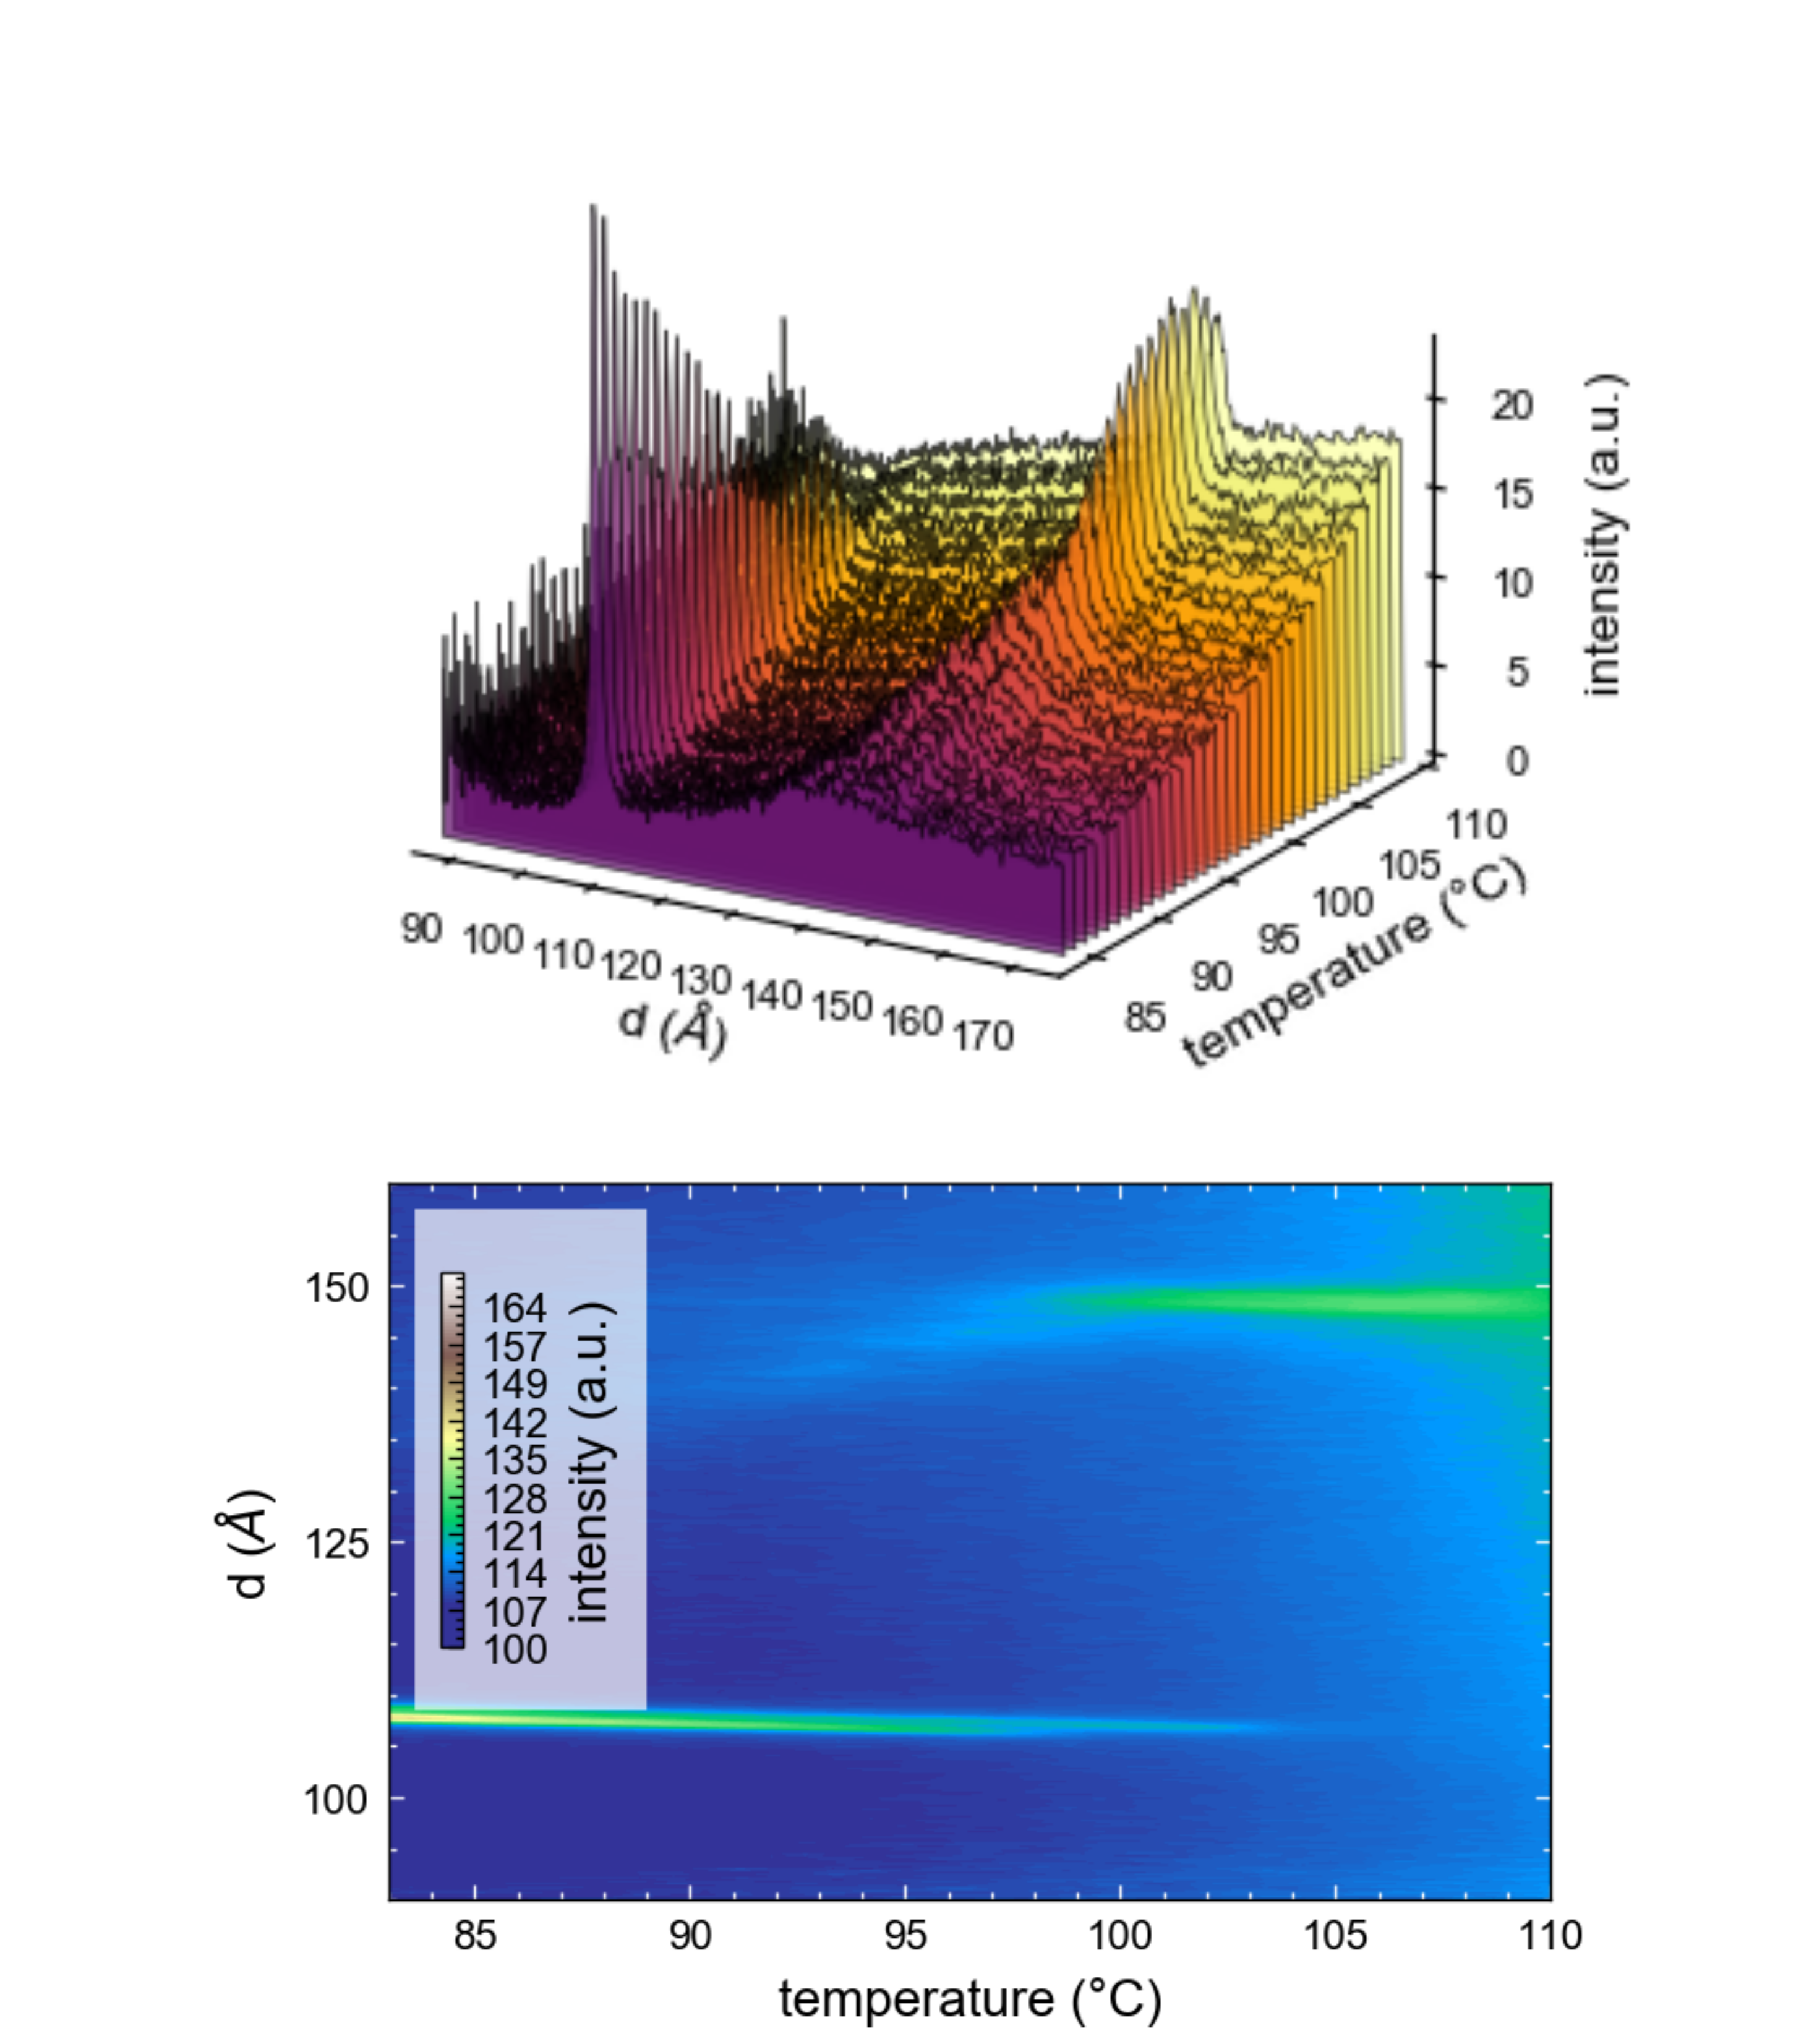
\includegraphics[width=.8\textwidth]{figs/pal30/rsoxssm2/sm2-rsoxs.png}
    \caption{\label{fig:pal30:diffractVt} Temperature behaviour of the
    \smcpalpha{} phase plotted as a waterfall plot in (a), and as a contour plot
    in (b). A bilayer ($d=\SI{112}{\angstrom} =2d_0$) corresponds to the 2-layer
unit-cell structure of the \smcapa{} phase, which sits directly below the
\smcpalpha phase in temperature. The resonant peak corresponding to the
\smcpalpha{} phase at $d\approx\SI{150}{\angstrom}$ is direct evidence that the
\smcpalpha{} phase is not a classic B2-type phase.}
\end{figure}


Below \SI{99}{\degreeCelsius}, the incommensurate peak broadens dramatically and
moves to higher $q$, indicating the presence of short-ranged, Sm2-like helical
fluctuations persisting in the Sm3 phase, and disappears at the transition to the Sm4
phase at \SI{83}{\degreeCelsius}. The Sm4 phase exhibits only the bilayer RSoXS
reflection at $q_B$.

\begin{figure}
    \centering
    \includegraphics[width=.6\textwidth]{figs/pal30/fromPaper/finalFigs/xray-combined.png}
    \caption{\label{fig:xray-results}X-ray scattering from \nfour{phi}.
        (a) SAXS gives a peak from the smectic layer ordering at $q=q_0$.
        The RSoXS peak at $q_H$ indicates that there is superlayer orientational ordering with periodicity $d_H$
        in the Sm2 phase.
        In general, superlayer orientational modulation in a smectic generates RSoXS peaks at wavevectors along the layer normal at
        $q(l,m) = l(2\pi/d_0) \pm m(2\pi/d_H)$\cite{levelut1999tensorial}.  The
        observation of an RSoXS reflection at $q = q(0,1)$ and the absence of an Umklapp peak at $q = q(1,-1)$  in
        the Sm2 confirms a superlayer helix with a scattering amplitude
        modulation due to the smectic layering that is undetectably weak.
        (b) Temperature dependence of resonant scattering. The helix peak at $q_H \approx1/(2.8 d_0)$ becomes diffuse in the Sm3 phase. Splitting
        of the bilayer peak at $q_B$, which would indicate helical precession of the bilayer structure, is not observed.
        }
\end{figure}


The RSoXS scattering from a single layer can be analyzed, following Levelut and
Pansu, in terms of a monoclinic second-rank tensor with a principal
axis tilted from and then azimuthally rotated about the layer normal~\cite{levelut1999tensorial,gleeson_resonant_2006,Barois2012review}.   Scattering
from a stack of such layers is calculated by summing over the contributions of the individual layers at different $z$.
Resonant scattering peaks from azimuthally
periodic arrangements are found at wavevectors along $z$, $q(l,m) = l(2\pi/d_0)
\pm m(2\pi/p)$, where $p$ is the pitch.  In principle, resonant
scattering should appear at all values of $l$ (harmonics of $q_0$), and at values
of $m=0,\pm1,\pm2$ that depend on the superlayer structure.  In an incommensurate, helical
structure, like the SmC$_\alpha$ phase, only the fundamental and harmonic peaks at
$q(l=0,m=+1,+2)$ and the Umklapp peaks at
$q(l=+1,m=-1,-2)$ are found in the range $0 < q(l,m) <
q_0$. If the resonant scatterers are confined to lie precisely on layers spaced
by $d_0$, then the intensities of these peaks will be identical~\cite{levelut1999tensorial}.
Out-of-layer molecular positional fluctuations, and, in particular,
those for which there is a coupled azimuthal orientation that keeps the molecule
on the helix, $\delta \phi = (2\pi/p)\delta z$, reduce the intensities of the
resonant harmonic peak
at $2q_H$ and of the Umklapp peaks at $q_0 \pm q_H$, relative to that of the fundamental at
$q_H$~\cite{levelut1999tensorial}. In our RSoXS scans of these peaks, only the
fundamental is seen above the background, so that only the upper limit of
the intensity ratio of the Umklapp and fundamental peaks
can be estimated. From the RSoXS heating scan of
Figure~\ref{fig:xray-results}(a), we find $I_\text{U}/I_\text{F} \lesssim 0.03$, implying a very
weak fractional modulation of the density of helical scatterers, $\rho$, due to fluctuations in the
smectic layering $\sqrt{\langle\delta\rho^2\rangle}/\rho_0 < 0.17$. The absence of the harmonic peaks places a similar limit on how much the density modulation of helical scatterers deviates from being purely sinusoidal.

\subsection{Optical Textures}
The optical textures of planar-aligned (bookshelf) cells of
\nfour{phi} were studied using PLM.
Upon cooling from the isotropic, the Sm1 phase grows in (at \SI{175}{\degreeCelsius})
as b\^{a}tonnets, giving a smooth, focal-conic texture typical of an orthogonal
fluid smectic (Figure~\ref{fig:main}(f), \autoref{fig:pal30:sm1:planar}).
\begin{figure}[h!]
    \centering
    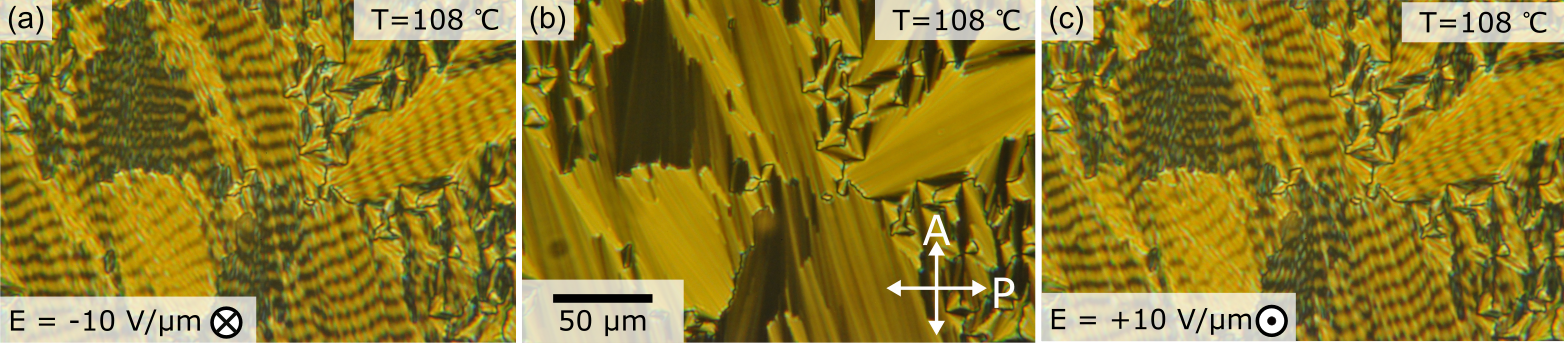
\includegraphics[width=\textwidth]{figs/pal30/textureSM1/sm1Textures100.png}
    \caption{\label{fig:pal30:sm1:planar} Planar aligned textures of Sm1. (a)
        Applied field out of the page, (b) ground state (no field), (c) applied
    field into the page.}
\end{figure}

However, given the large value of the estimated
molecular tilt, $\theta_\textrm{xray}$, the Sm1 is probably a de Vries
smectic.
In planar-aligned cells, there is no observable field-induced change of the in-plane birefringence, $\Delta n= n_\parallel
-n_\perp$, in small applied electric fields  (Figure~\ref{fig:main}(f)),
or in the optic axis orientation, $\theta_\text{opt}$ (Figure~\ref{fig:threshold}).

Below \SI{115}{\degreeCelsius}, a threshold field, $E_\text{th}$, above which a first-order structural change marked by the appearance of chiral conglomerate domains occurs, becomes experimentally accessible.
These domains are polar and exhibit a uniform, saturated optic axis tilt on the
order of $\theta_{\rm opt} \approx \SI{18}{\degree}$ from the layer normal, implying that the achiral, untilted Sm1 phase
transforms in the field to a B2-like, homochiral \smcspf{phi} state (Figure
S1(c))~\cite{eremin2008electrically}. The field-induced left- and right-handed domains form a ``tiger stripe''
pattern (Figures~\ref{fig:main}(e,g)). 


The local domain handedness in this unusual conglomerate texture
is apparently locked in after the first few field cycles.  This bias is due to a chiral
memory effect at the surface since, as
Figures~\ref{fig:main}(d)~and~\ref{fig:threshold} show, the
sub-threshold bulk state has an achiral field response, with a linear polarization current (implying $P \propto E$) and no
detectable reorientation of the optical tilt.
$E_\text{th}$  decreases strongly on cooling as the transition to the Sm2 phase is approached, as shown in the inset of Figure~\ref{fig:threshold}.
%
\begin{figure}[h!]
    \centering
    \includegraphics[width=.6\textwidth]{figs/pal30/fromPaper/finalFigs/threshold-inset2.png}
    \caption{\label{fig:threshold}
        Optical tilt of \nfour{phi} vs.\ applied field. The Sm1
        phase shows no electrooptic response in weak fields $E<E_\text{th}$. Fields $E>E_\text{th}$ induce an electroclinic
        tilt and result in the formation of chiral domains.
        $E_\text{th}$, which becomes smaller with decreasing $T$ (inset), matches
        closely $E_\text{sat}$, the field at which the induced
        polarization saturates, extracted from Figure~\ref{fig:main}(d).
        The Sm2 phase exhibits a chiral
        electroclinic effect near $E=0$ and hysteresis in the field-induced helix unwinding to the
        \smcspf{phi} state.   }

\end{figure}


In the lower part of the Sm1, and throughout the Sm2, Sm3 and Sm4 phases, the birefringence increases on application of an electric field, as seen in Figure~\ref{fig:main}(c),  changing from yellow to orange.
Measurements of $\Delta n$ at $E = 0$ and $E = \SI{20}{\volt\per\micro\metre}$
(Figures~\ref{fig:main}(c) and S6),
show that the birefringences in the lower temperature
phases with and without an applied field are of the order of $\Delta n_\text{on} \sim 0.12$ and $\Delta n_\text{off} \sim 0.10$.
Assuming that the field-on \smcspf{phi} state
(Figures~\ref{fig:main}(n--p) and S1) gives a uniform
director orientation with the optic axis in the plane of the cell, then $\Delta
n \sim 0.12$ would correspond to the maximal birefringence $n_3-n_1$ of the
\smcspf{phi} state. Modeling the bent-core molecule
as two uniaxial, birefringent rods connected with an opening angle of
$\Psi$, and tilting this molecule from $z$ by an angle $\theta$,
we have calculated the birefringence of all of the states shown in
Figure~\ref{fig:main}. If the Sm1 phase is assumed to be a de Vries SmA, with
azimuthally averaged molecules distributed on a tilt cone of angle
$\theta$, the best fit to the measured birefringence values $\Delta n_\text{on}$ and $\Delta n_\text{off}$ is
obtained with $\Psi = \SI{150}{\degree}$ and $\theta = \SI{15}{\degree}$.
The calculated birefringence as a function of temperature is shown in Figure~S6.
\begin{figure}[h!]
    \centering
    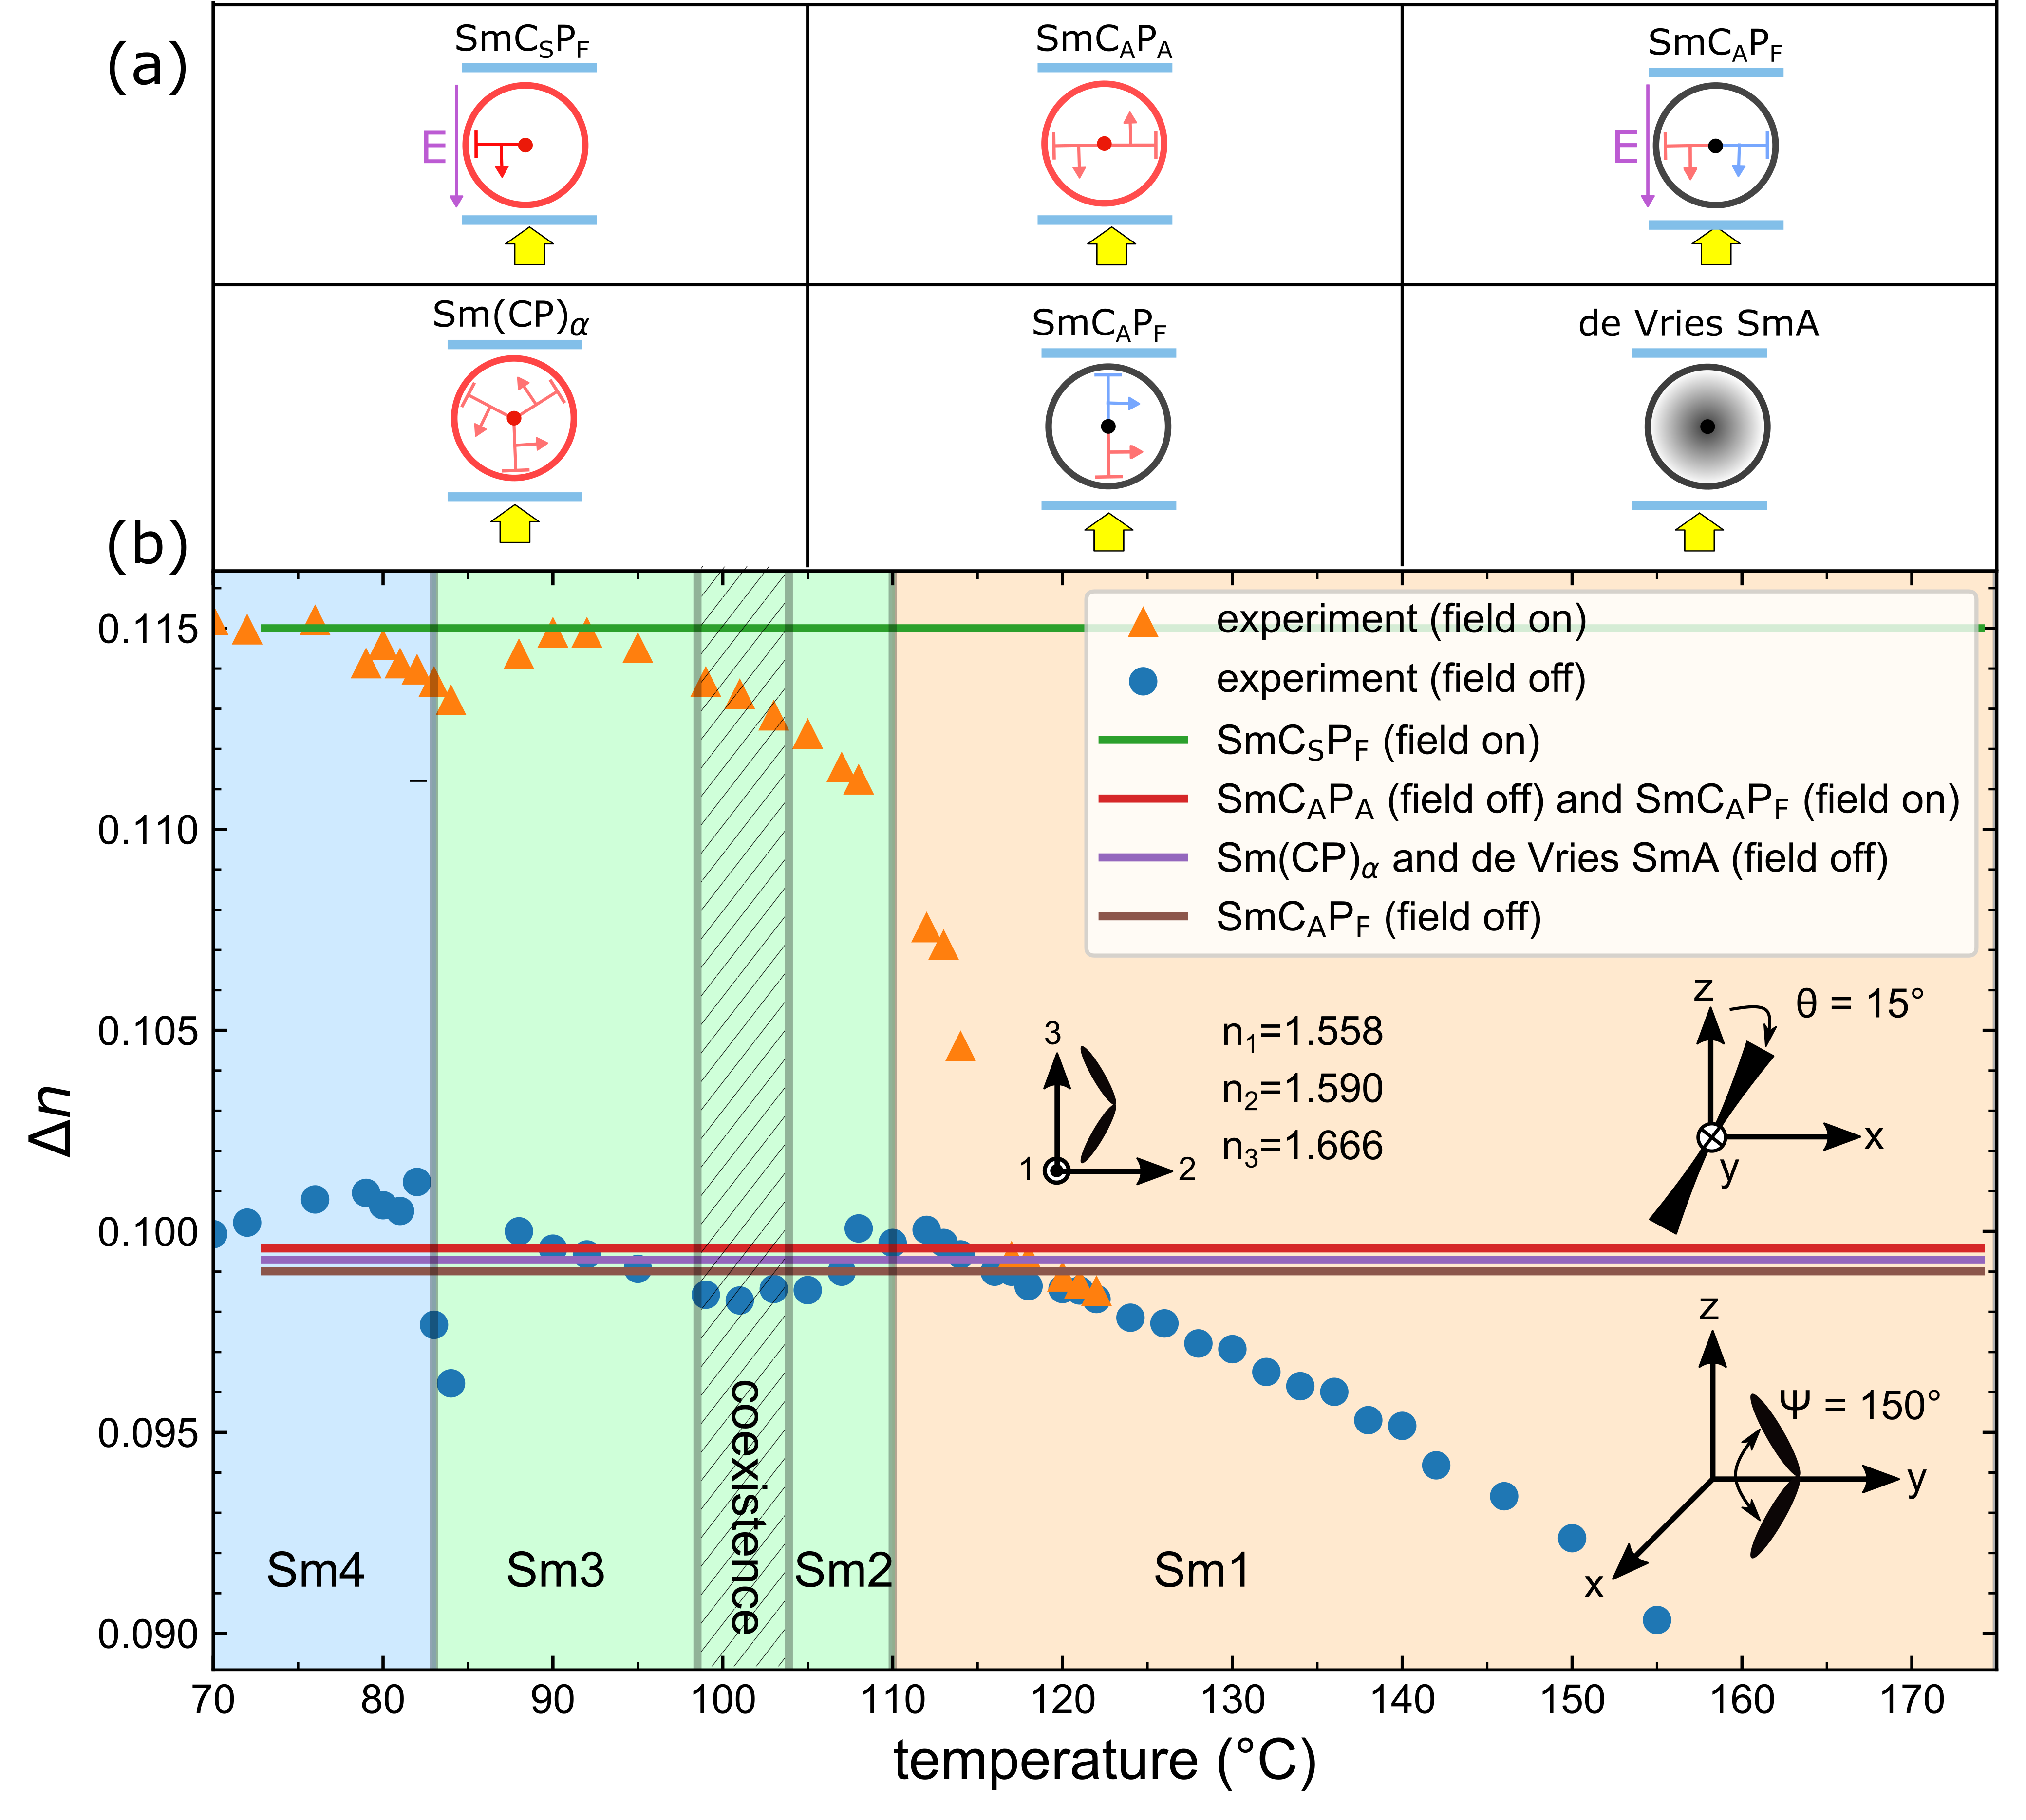
\includegraphics[width=.8\textwidth]{figs/pal30/fromPaper/finalFigs/theory-biref.png}
    \caption{\label{fig:pal30:theorybiref} Calculated birefringence of \nfour{},
        assuming Boulder phase assignments,
    shown as a function of temperature}
\end{figure}


The transitions between the smectic phases are difficult to see when $E=0$ because they are all orthogonal in appearance,
with an optic axis along $z$, and have similar birefringence.
At the transition from Sm1 to the Sm2 phase,  however, arbitrarily small electric fields induce molecular tilt in the
(Figure~\ref{fig:threshold}), leading to the formation of optically distinct, conglomerate chiral
domains with opposite tilt (Figures~\ref{fig:main}(h--j)), again
corresponding to a field-induced transition to a \smcspf{phi} state.
The birefringence and orthogonal appearance of the Sm2 ground state are consistent with
the helical superlayer structure indicated by RSoXS.

\begin{figure}[h!]
    \centering
    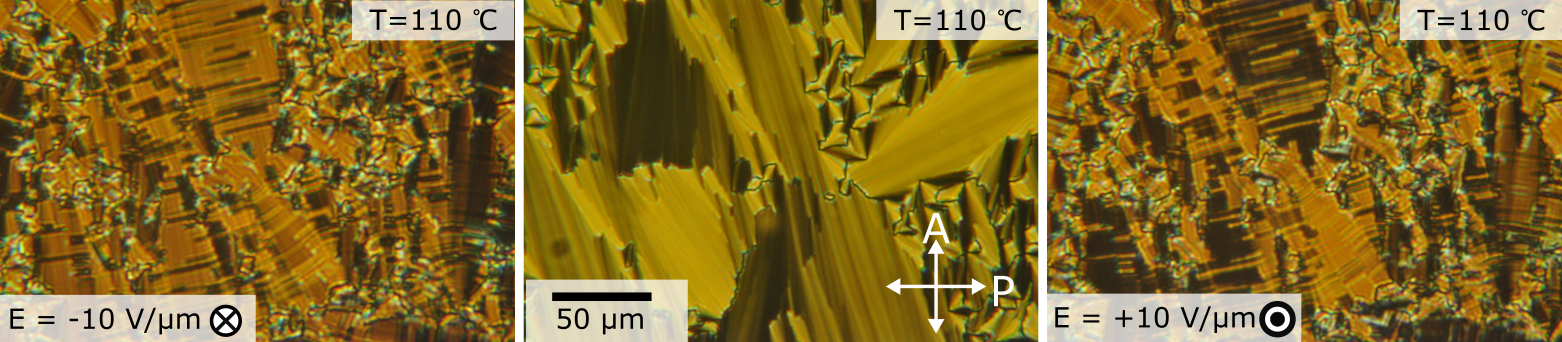
\includegraphics[width=\textwidth]{figs/pal30/textureSM2/sm2Textures100.png}
    \caption{\label{fig:pal30:planar-textures} Textures of both the
        Sm2 (\smcpalpha{}) and Sm3 (\smcapa{})
    phases of \nfour{}: reminiscent of a \smcapa{} texture. }
\end{figure}


The texture and birefringence of the Sm3 phase in the absence of field are consistent with the \smcapa{phi} bilayer structure indicated by RSoXS.
The field-induced conglomerate domain morphology in both the Sm2 and Sm3 phases is distinct from that of the undulating Sm1
tiger stripes, with straight
domain boundaries that tend to form parallel to the layers, as in an
antiferroelectric calamitic being driven to a ferroelectric
state~\cite{li1995reversible}.
The optical tilt in these domains is found to be $\theta_\mathrm{opt}\sim 18^\circ$.
\begin{figure}[h!]
    \centering
    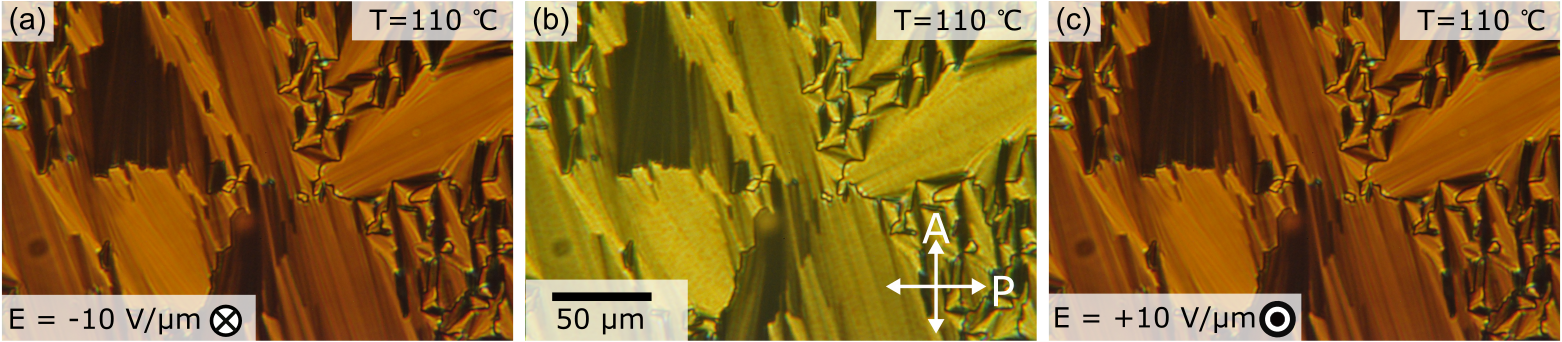
\includegraphics[width=\textwidth]{figs/pal30/texturesm4/sm4Textures100.png}
    \caption{\label{fig:pal30:planar-textures} Textures of both the
        Sm2 (\smcpalpha{}) and Sm3 (\smcapa{})
    phases of \nfour{}: reminiscent of a \smcapa{} texture. }
\end{figure}


The response to applied field changes dramatically again at
the transition from Sm3 to Sm4, with no visible brush rotation or evidence of domain formation at any $E$. 


The birefringence in the Sm4 phase increases continuously with field, saturating at a value comparable to that observed in the field-induced Sm2 and Sm3 conglomerate domains.

\subsection{Polarization Current}

The polarization current, measured with a triangular
applied field, for the entire phase sequence is shown vs.\ temperature in Figures~\ref{fig:main}(d)
\autoref{fig:pal30:prcBig}. The polarization current will be discussed in order
of cooling.

\begin{figure}[h!]
    \centering
\includegraphics[width=\textwidth]{figs/pal30/fromPaper/finalFigs/polzv9.png}
\caption{\label{fig:pal30:prcBig} Polarization current of \nfour{} shown as a
function of the applied field strength.}
\end{figure}



Upon cooling from the isotropic, a single current bump centered
about $E=0$ first appears at lower temperatures in the Sm1 phase, indicating a Langevin-type
field-induced orientation of $\mathbf{P}$, with a linear response near $E=0$
and the current vanishing  when $\mathbf{P}$ becomes saturated (for $E \ge E_\text{sat}$).

\begin{figure}[h!]
    \centering
    \includegraphics[width=\textwidth]{figs/pal30/prc/3dplot-sm1.png}
    \caption{\label{fig:pal30:sm1:prc1} Zoomed in polarization current measurements for \nfour{} in the high temperature
    Sm1 phase.}
    \end{figure}
 

Significantly, $E_\text{sat}$ is similar in magnitude to $E_\text{th}$, the threshold
field required for the Sm1
transition to chirality observed optically (\autoref{fig:threshold}, inset), indicating that the
field first orders the Langevin system of initially azimuthally random molecular
polarizations, with the Sm1 remaining in an achiral state, and that the phase becomes
chiral only at higher fields, once $\mathbf{P}$ is saturated (Figure S10). 

\begin{figure}[h!]
    \centering
    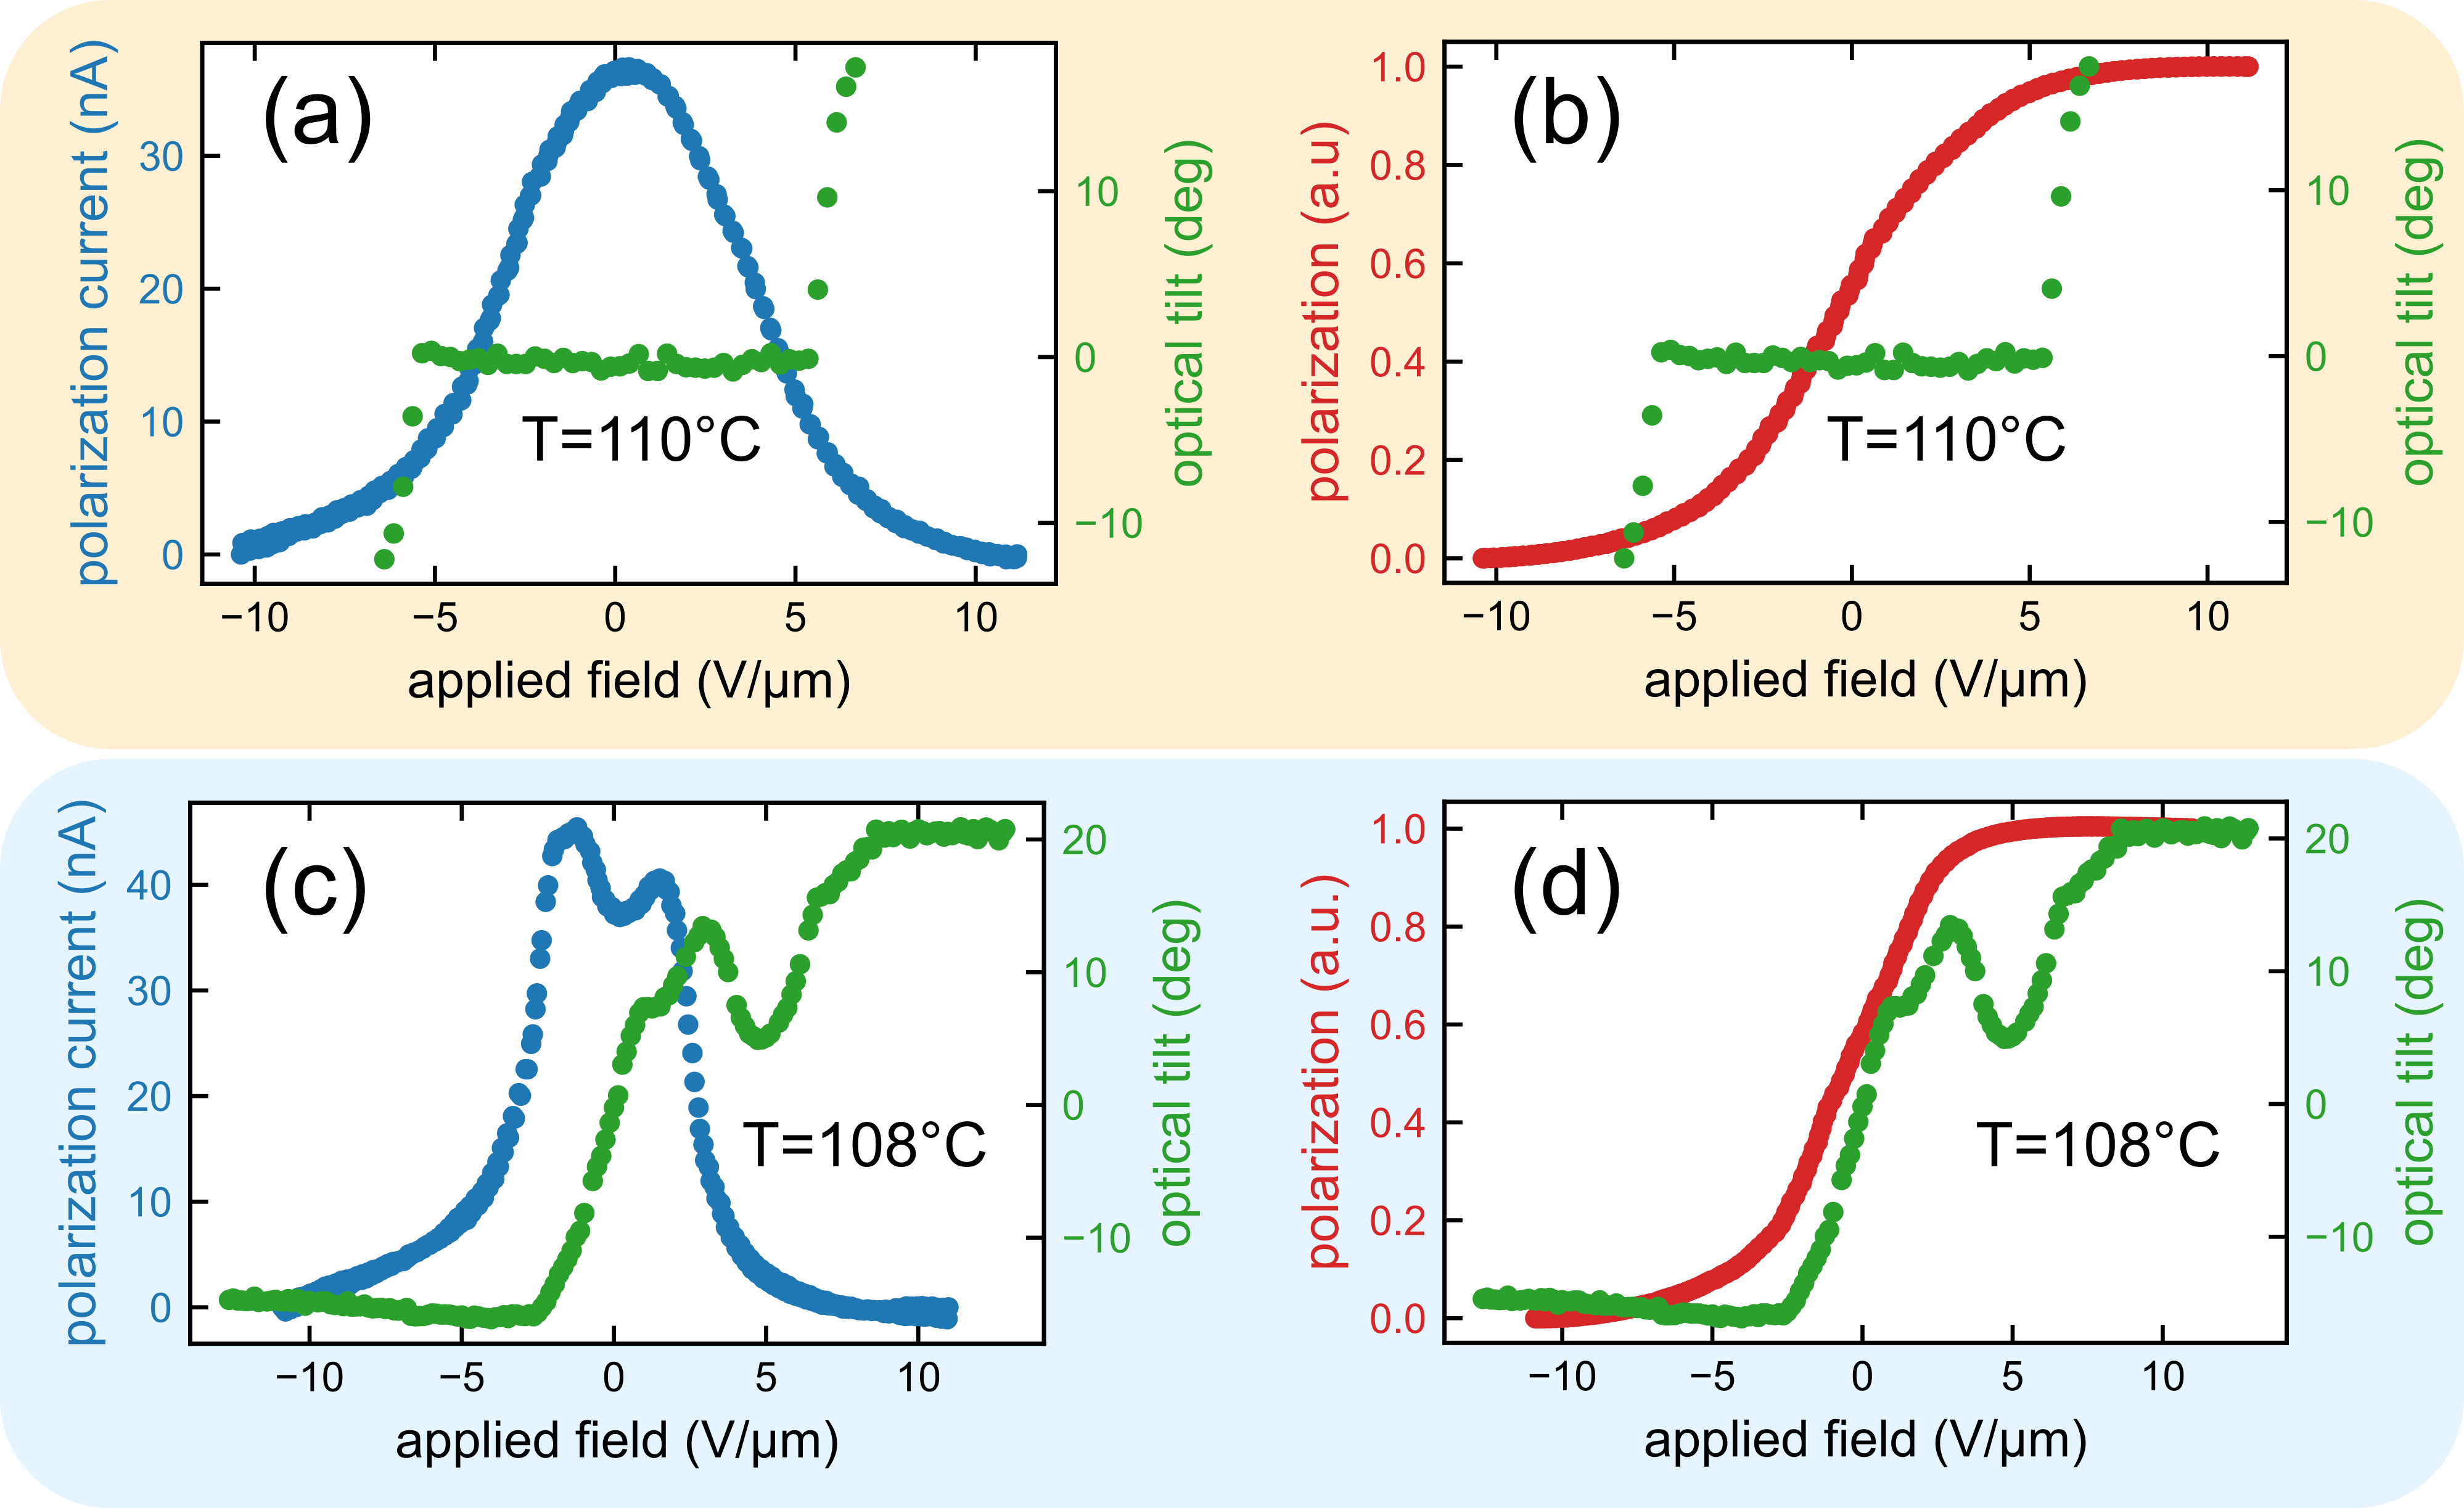
\includegraphics[width=.6\textwidth]{figs/pal30/prc/PRCvsTilt/PRCVtilt.png}
    \caption{\label{fig:pal30:prcvtilt} The polarization current and the optical
    tilt plotted as a function of applied field strength for both the Sm1
(de Vries SmA) (a,b) and the Sm2 (\smcpalpha{}) (c-d). The polarization current
has additionally been integrated to calculate the time-dependant net
polarization. The threshold electric field ($E_\textrm{th}$) required to manifest the tiger-stripes can
be directly read from the green curve denoting the optical tilt (for
T=\SI{110}{\degreeCelsius}, $E_\textrm{th} \approx \SI{5}{\volt\per\micro\metre}$),
and the saturation electric field where the net polarization is no longer
changing ($E_\textrm{sat}$) can be directly
read from the red curve, which denotes the net polarization, (for
T=\SI{110}{\degreeCelsius}, $E_\textrm{sat} \approx \SI{5}{\volt\per\micro\metre}$).
Both $E_\textrm{th}$ and $E_\textrm{sat}$ are plotted in as the inset of
\autoref{fig:threshold}. }
\end{figure}


On cooling to the Sm2 phase, the polarization bump splits into three peaks roughly centered about
$E=0$ that evolve to two peaks on cooling through the Sm3, shown in
\autoref{fig:pal30:sm2:prc2}.


\begin{figure}[h!]
    \centering
    \includegraphics[width=\textwidth]{figs/pal30/prc/3dplot-sm2.png}
    \caption{\label{fig:pal30:sm2:prc2} Polarization current of sm2 of \nfour{}
    plotted against applied voltage}
\end{figure}
\nfour{phi} thus transforms on cooling from the non-polar
Langevin ground state of the Sm1, where $P=0$ is enforced by entropy, to energetically stabilized ground
states in which the spatial average of
$\mathbf{P}(\mathbf{r})$ in the absence of applied field is also zero: the incommensurate helical winding of the
polarization
in the Sm2, and the antiferroelectric bilayer structure in the Sm3.




At the
transition to the Sm4, a single current peak dominates, characteristic of the block
polarization switching of a ferroelectric ground state that is surface-stabilized
with $\mathbf{P}$ parallel to the cell plates at $E=0$, such as occurs in the orthorhombic \smapf{phi} phase~\cite{shen2011effective}.

\begin{figure}[h!]
    \centering
    \includegraphics[width=\textwidth]{figs/pal30/prc/3dplot-sm34.png}
    \caption{\label{fig:pal30:sm34:prc1} Polarization current measurements for \nfour{} in the high temperature
    Sm1 phase.}
    \end{figure}
 
The absence of brush rotation during the field-induced reorientation of the
polarization in Sm4 is consistent with achiral \smcapf{phi} superlayer organization.

\section{Results and Discussion}

In summary, X-ray and optical experiments show that \nfour{phi}, an achiral, bent-core mesogen, forms smectic
liquid crystal phases with the molecules substantially tilted from the layer
normal, with phase sequence:
$$
    \resizebox{.8\textwidth}{!}{$\text{I} \xrightarrow{
        175\si{\degreeCelsius}} \textrm{de Vries SmA} \xrightarrow{
    110\si{\degreeCelsius}} \textrm{Sm(CP)}_\alpha\xrightarrow{99\si{\degreeCelsius}}
    \smcapa{}
    \xrightarrow{83\si{\degreeCelsius}}\smcapf{}\xrightarrow{65\si{\degreeCelsius}}
\text{Cr}$.}
$$
The highest temperature phase exhibits short-ranged ordering of the
tilt azimuth that is decoupled from the molecular polarization, forming a uniaxial, non-polar, achiral
de Vries smectic A.  An applied electric field of increasing magnitude
continuously aligns the initially random polarization and the phase acquires orthorhombic symmetry. The field eventually saturates the
polarization orientation, inducing a transition to a tilted, chiral, ferroelectric
smectic state.  
\begin{figure}[h!]
    \centering
    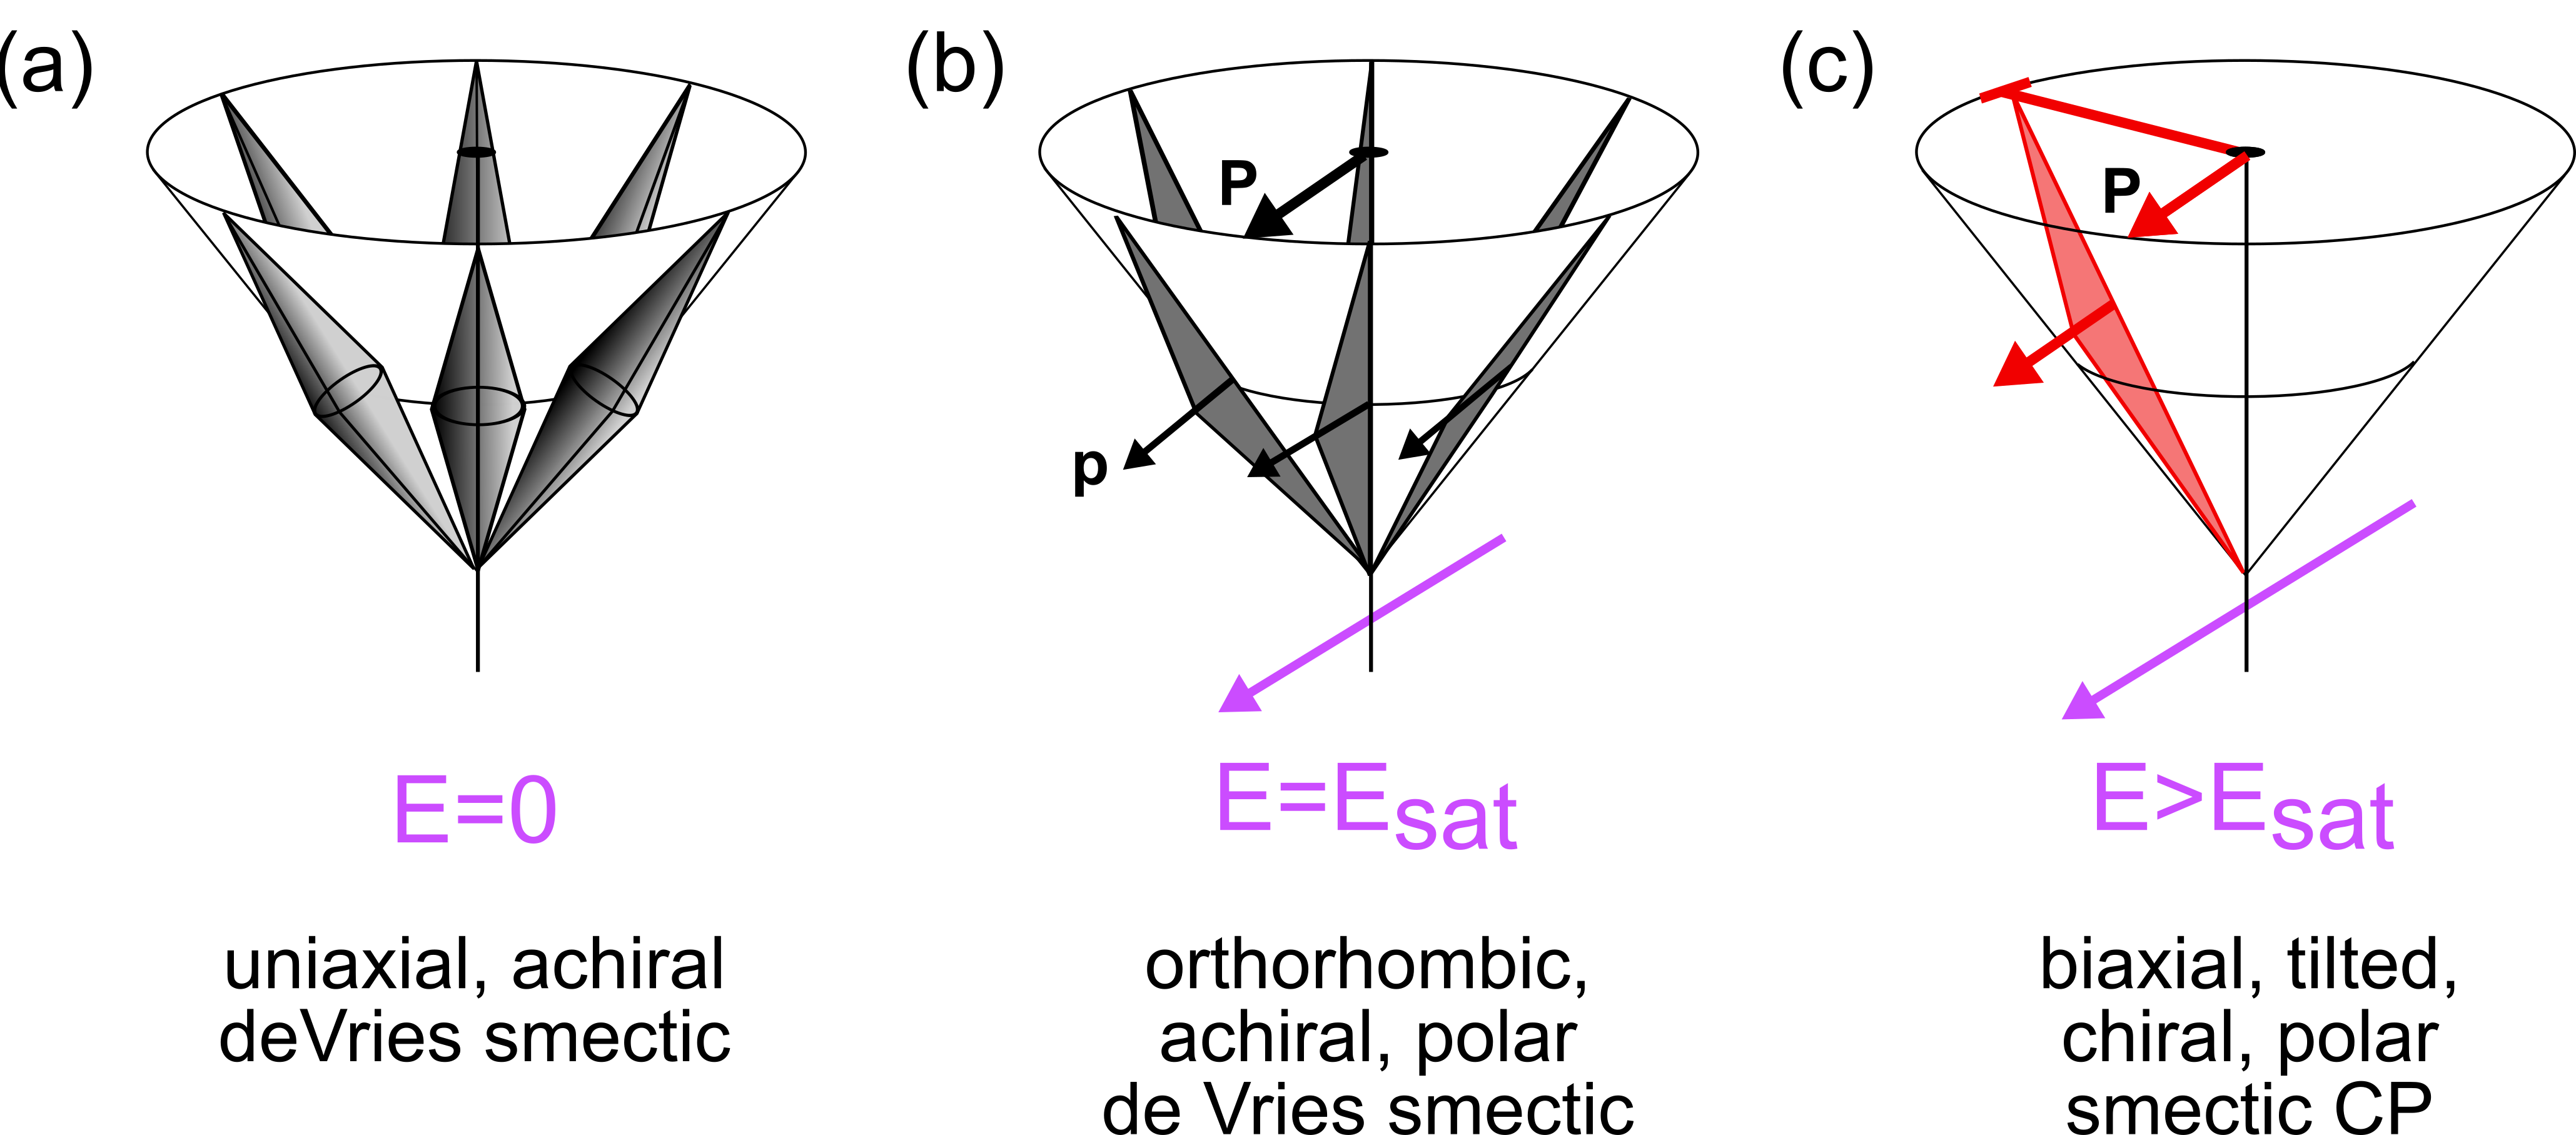
\includegraphics[width=\textwidth]{figs/pal30/fromPaper/finalFigs/dvAlign.png}
    \caption{\label{fig:pal30:sm1:align} Evolution of de Vries SmA bent-core
    phase under the application of a field}
\end{figure}

Upon cooling, a novel chiral, ferrielectric phase which we call
the \smcpalpha{phi} appears.
This phase is similar to the SmC$_\alpha$ phase of chiral, rod-shaped molecules
\cite{mach_structural_1998,mach_structures_1999,hirst2002interlayer,huang2015liquid},
but with the chirality appearing here as a broken symmetry.
A periodic azimuthal precession of the director about the layer normal that is incommensurate with the
smectic layering is confirmed by the presence of Bragg reflection peaks in
carbon-edge resonant soft X-ray scattering. The absence of the corresponding
resonant Umklapp peak unambiguously identifies this structure as a helical
modulation of the orientational ordering in which molecules exhibit substantial coupled
rotational/positional out-of-layer fluctuations, forming a
twist-bend-like helix.


\end{document}

%\section{A Brief History of Chirality in Bent-Core Smectics}
%
%
%\subsection{Conventional Phase of \nfour{phi}}
%
%To briefly recap Section~\ref{test}, the low-temperature phases of \nfour{} are conventional B2
%phases: the \smcapa{} and the \smcapf{}. 
%The conventional representation of the polarization current for the Sm3 and Sm4
%phases are shown in \autoref{fig:pal30:sm34:prc1}.
%
%
%\begin{figure}[h!]
%    \centering
%    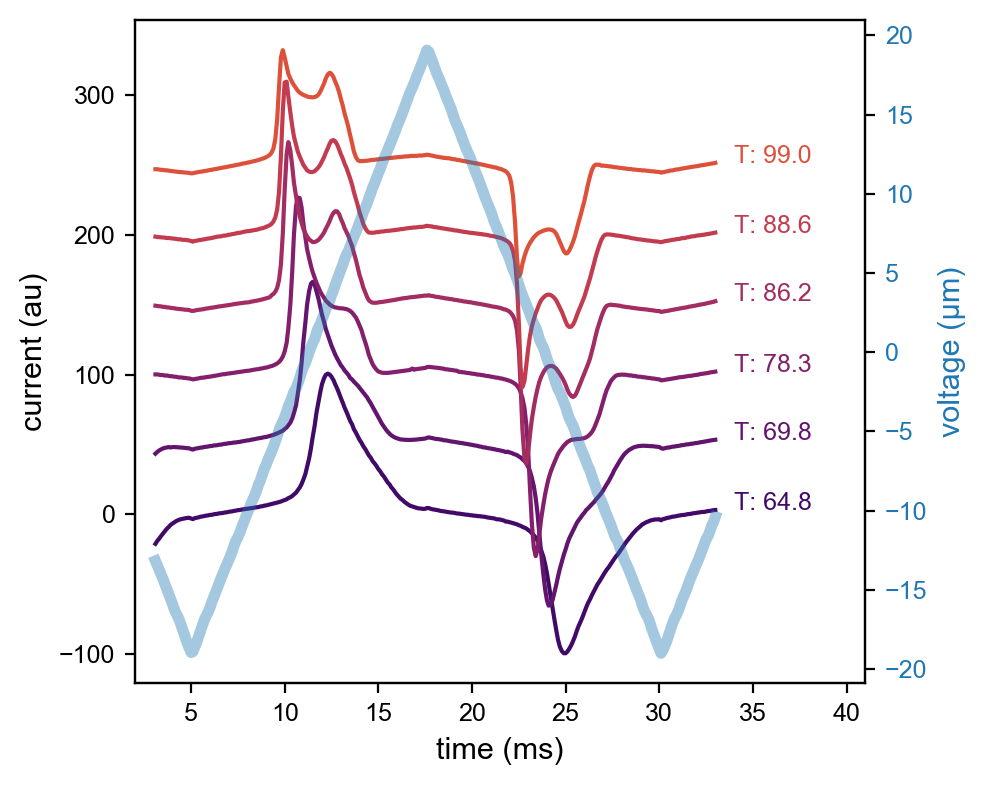
\includegraphics[width=.8\textwidth]{figs/pal30/prc/spacedSmRPRC.png}
%    \caption{\label{fig:pal30:sm34:prc1}}
%\end{figure}
%However, it the switching dynamics of the phases become more clear if the
%polarization current is plotted directly against the driving voltage, shown in
%\autoref{fig:pal30:sm34:prc2}
%
%\begin{figure}[h!]
%    \centering
%    \includegraphics[width=\textwidth]{figs/pal30/prc/3dplot-sm34.png}
%    \caption{\label{fig:pal30:sm34:prc2}}
%\end{figure}
%
%This is the end of this section.
%
%
%\section{Characteristics of the \smcpalpha{} phase}
%
%
%
%\subsection{The \nfour{} Molecule and Phases}
%\todo{add phase description with Sm2} Go bottom up, to get the boring phases out
%of the way. (maybe put this in the introduction of \nfour{})
%\subsection{Textures of the \smcpalpha{} phase}
%\subsubsection{Planar Aligned Textures}
%As discussed in Section~\ref{sec:intro:pl-aligned}, in planar-aligned cells, the
%optic axis of the liquid crystal is perpendicular to the $\vec{k}$ of the
%applied light--meaning we will be sensitive to relative orientations of the
%long-axis.
%
%In \autoref{fig:pal30:planar-textures}, the planar textures of the Sm2 phase of \nfour{} are shown.
%Comparing these with previously published textures reveals a strong similarity
%to the \smcapa{}
%phases\cite{link_spontaneous_1997,ReddyInfluencefluorinesubstituent2003}. As
%discussed in Section~\ref{sec:intro:pal30-phases}, the \nfour{} phase directly below the
%Sm2 is a \smcapa{}, but with strikingly long-range and regular conglomerate
%chiral structure, where the handedness is grouped together into stripes. There
%exists no clear phase transition in the textures between the Sm2 and Sm3 in
%planar aligned cells.
%
%\begin{figure}[h!]
%    \centering
%    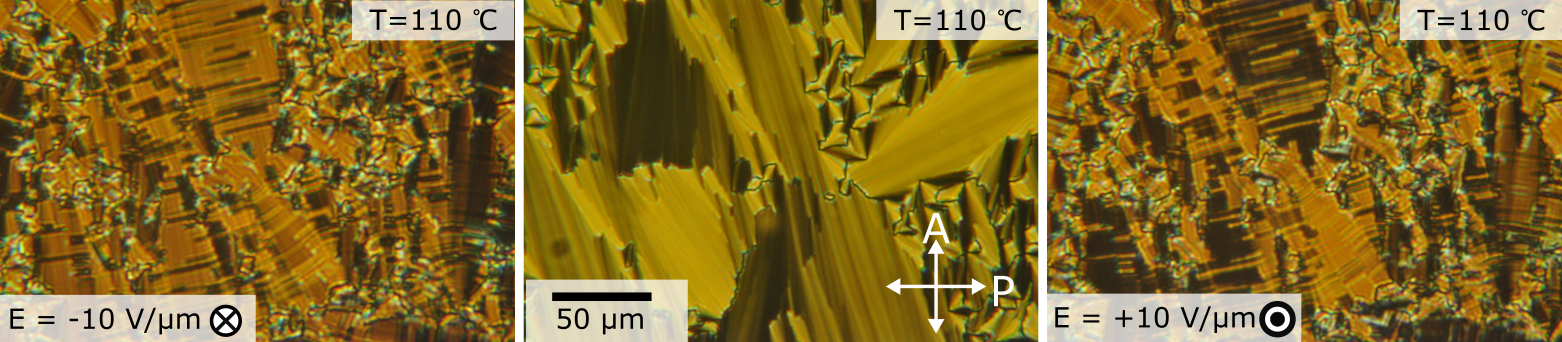
\includegraphics[width=\textwidth]{figs/pal30/textureSM2/sm2Textures100.png}
%    \caption{\label{fig:pal30:planar-textures} Textures of the \smcpalpha{}
%    phase of \nfour{}: reminiscent of a \smcapa{} texture.  }
%\end{figure}
%
%This similarity is due to the fact that, broadly, the \smcapa{} and
%\smcpalpha{} phases are identical optically. Both phases have unit-cells whose dielectric tensor is uniaxial (where
%the $\epsilon_{xx} = \epsilon_{yy}$), so the optic axis will be parallel to the
%layer normal and the texture appears like a SmA in it's ground state.
%
%Both phases are polar, so with a high enough field both states will switch into
%an aligned \smcspf{} state, which gives a birefringent contrast between domains with different handedness. This contrast is
%because of the synclinic nature of the \smcspf{} phase--- because the tilt is
%now aligned between the subsequent layers, the phase can organize into
%conglomerate chiral domains with the optic axis tilted with respect to the layer
%normal.
%\todo{figure describing this switching mechanism}
%
%We can directly measure the optical tilt in the switched state, by simply
%rotating the stage when a field has been applied such that an initially dark
%stripe becomes completely bright. The angle of this rotation is
%$2\theta_{opt}$. To observe the tilt dyanamics, we have to extend this analysis
%as we cannot rotate a stage at the \SI{20}{\hertz} frequency that these samples
%usually switch at.
%
%We can extract a measurement of the dynamic optical tilt, $\theta_\textrm{opt}$, by
%examining the contrast between the bright and dark regions of the stripe.
%Knowing that the brightness of a birefringent material viewed under cross
%polarizers is $I \propto \sin(2\theta)^2 $, the contrast between a ``bright''
%and adjacent ``dark'' stripe is given by:
%\begin{align}
%    C = \delta I = I_\textrm{bright} - I_\textrm{dark} &= \sin(2\theta_b)^2 -
%    \sin(2\theta_d)^2 \\
%&= \frac{1-\cos(4\theta_b)}{2} - \frac{1-\cos(4\theta_d)}{2} \\
%&= -\sin(2i(\theta_d+\theta_b))\sin(2(\theta_d-\theta_b))
%\end{align}
%
%Because of the symmetry of the \smcspf{} state, we know that $\theta_d
%=-\theta_b$ (the magnitude of the tilt is equal, but the sign depends on the
%chirality).
%
%This allows to directly connect the contrast with the tilt angle:
%\begin{align}
%    \label{eq:contrast-tilt}
%    C \propto\sin(4\theta_\textrm{opt}).
%\end{align}
%
%This analysis assumes that the state we are measuring can be roughly
%approximated by a \smcspf{}. This will be a good approximation at high field
%strengths, but may be false at lower fields, where the helix of the \smcpalpha
%phase may be distorted, but not switched.
%
%Plotting the result in \autoref{fig:pcVtilt} we see thresholdless optical
%switching, where the contrast (optical tilt) increases linearly with applied
%field. Interestingly, the \smcpalpha phase accesses a `dark' state, which was
%also seen in homeotropic cells, shown in \autoref{fig:pal30:homeo}. This will be
%discussed in further detail in \autoref{sec:pal30:discussion}
%
%\begin{figure}[h!]
%    \centering
%    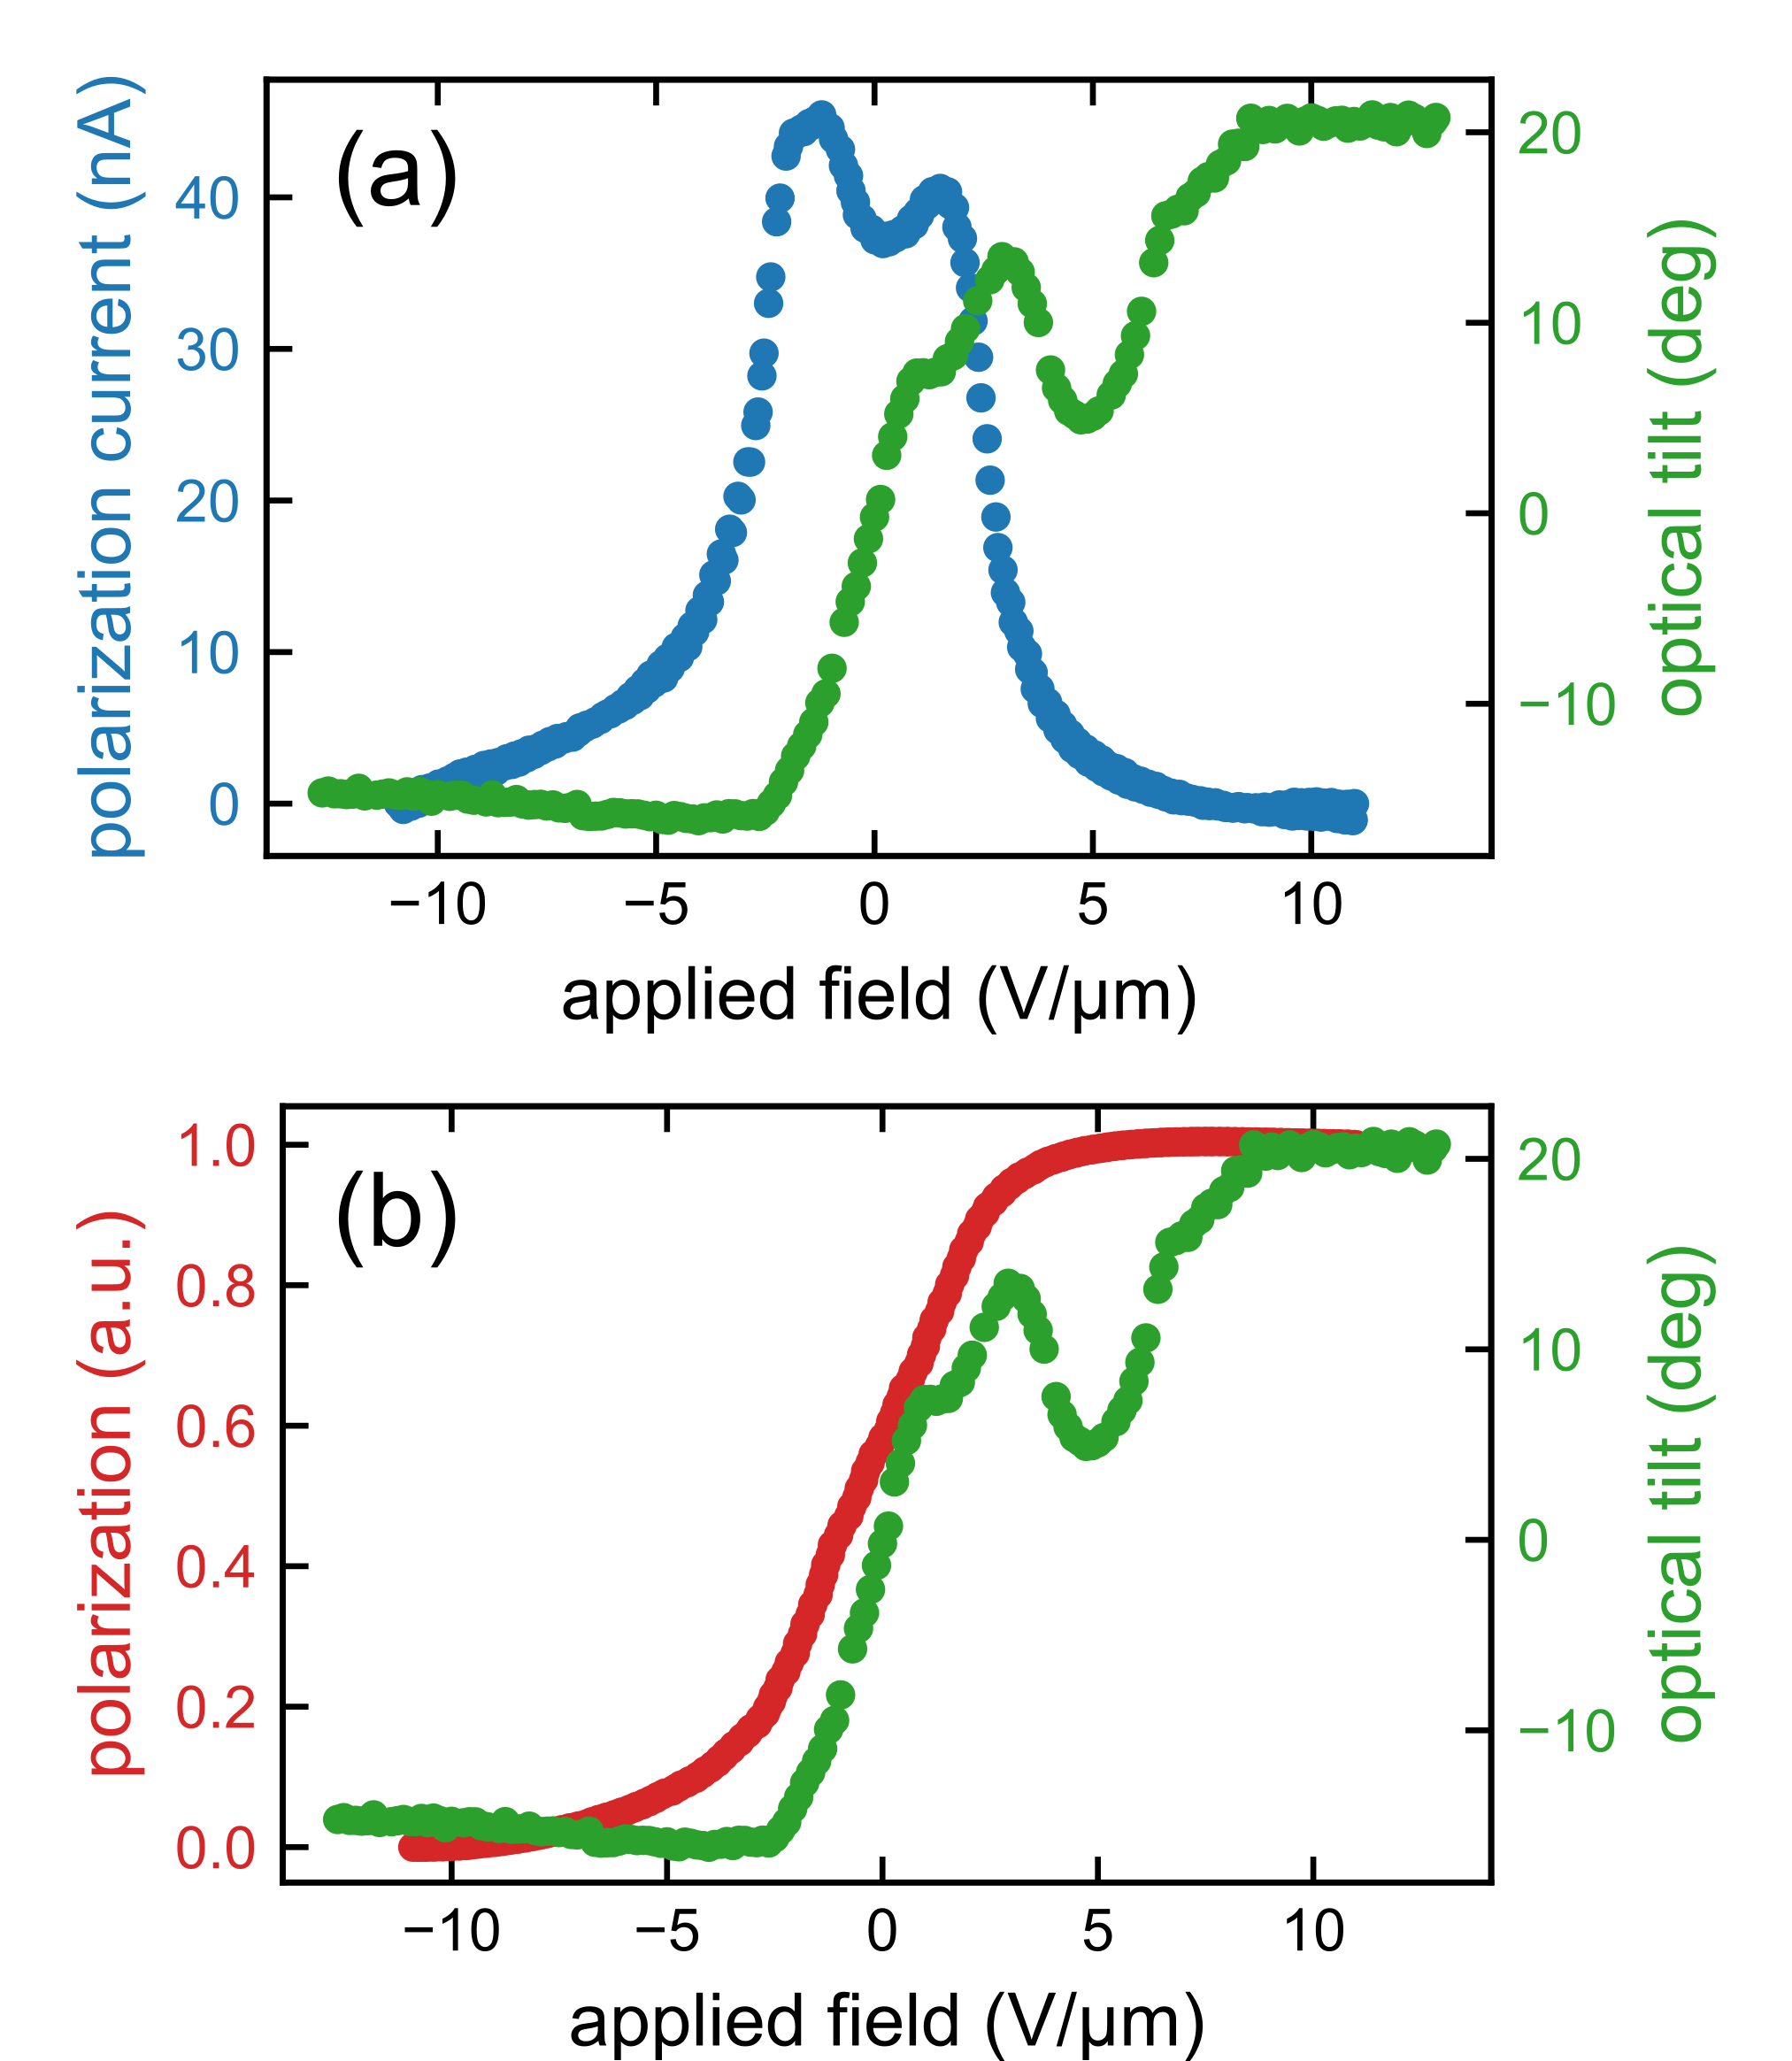
\includegraphics[width=.8\textwidth]{figs/pal30/prc/PRCvsTilt/T108.png}
%    \caption{\label{fig:pcVtilt} Dynamic optical tilt of \smcpalpha{}. On
%    application of a field, the state briefly passes through a `dark' state,
%where the contrast decreases.}
%\end{figure}
%
%
%In conclusion, the textures of the \smcpalpha{} phase have identical
%characteristics to those of the \smcapa{}, though an interesting dark state
%emerges when viewed under dynamic conditions. 
%
%\subsubsection{Homeotropic Aligned Textures}
%Though we were unable to achieve good homeotropic alignment, we can rely on the
%published results of the Dublin group, who published a series of papers on the
%\nfour{} homolog
%series\cite{panarin_sequence_2011,sreenilayam_properties_2012,SreenilayamOccurrenceFiveDifferent2015,sreenilayam_spontaneous_2016}.
%Though their interpretation is wrong (\nfour{} is not an orthogonal phase), they
%report beautifully aligned homeotropic textures and study the response of these
%textures to an applied in-plane electric field. These textures are reproduced from Sreenilayam et
%al\cite{sreenilayam_properties_2012} in \autoref{fig:pal30:homeo}.
%\begin{figure}[h!]
%    \centering
%    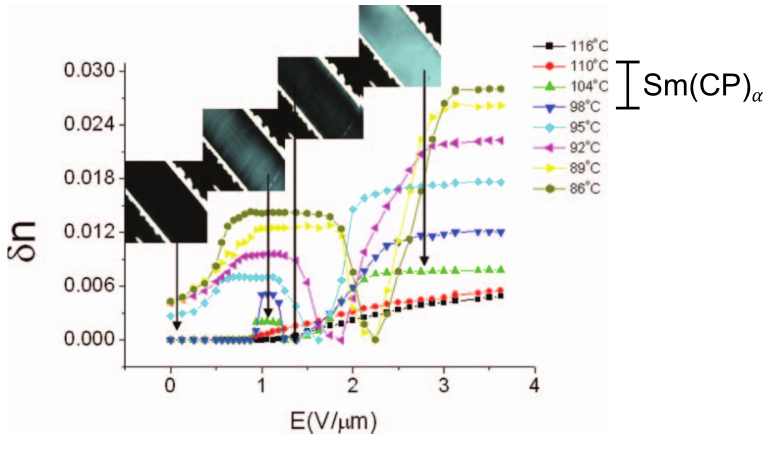
\includegraphics[width=.8\textwidth]{figs/pal30/fromPapers/textures/pal30-Homeo-2012-labelled.png}
%    \caption{ \label{fig:pal30:homeo} Homeotropic textures of \nfour{}. The relevant temperatures for the Sm2 phases are \SI{104}{\degreeCelsius}, and \SI{98}{\degreeCelsius}. The biaxiality in the Sm2 is distinguished by a small `hump' with small applied field, that gets larger on cooling, and changes in character on cooling through the Sm2$\rightarrow$Sm3 phase transition at \SI{99}{\degreeCelsius}, where it broadens. Reproduced from Sreenilayam et al\cite{sreenilayam_properties_2012}.}
%\end{figure}
%
%
%The phase of interest, \smcpalpha, occurs in the temperature range \SIrange{110}{99}{\degreeCelsius}. There is a clear change in the field-behaviour of the biaxiality at the Sm2$\rightarrow$Sm3 transition temperature. However, because these phases are tilted the authors original interpretation of the data needs to be revisited.  
%
%For our purposes, we can use these textures to distinguish the \smcpalpha{} phase
%from the closely related \smcapa{} phase. The \smcapa{} phase should be weakly
%biaxial in homeotropic cells. The anticlinic structure should 'average' out any
%anisotropy in the dieletric tensor due to the tilt of the molecule, but because
%these are bent-core phases, there is a built in anisotropy of the dielectric
%tensor due to the rotation symmetry breaking of the bananna structure, which
%should manifest in homeotropic cells as a schlieren texture that allows for $\pm
%1/2$ defects.
%
%From \autoref{fig:pal30:homeo}, it is clear that, for the temperature ranges of
%\smcpalpha, the textures appear dark-- they have no measurable biaxiality. This
%means that the inherent anisotropy of the dielectric tensor of the molecule
%\textit{must} be organized in a structure that averages it out. This is a clue
%to the helical nature of the \smcpalpha{}. 
%
%
%
%%The original interpretation, that there exists a `dark' intermediate state on application of the electric field ($\approx \SI{2}{\volts\per\micron}$), where the polarization of each layer is perpendicular to each other.
%        
%\subsection{Electro-Optic Behaviour of the \smcpalpha{} phase}
%We can study the electro-optic behaviour of \nfour{} in both homeotropic and
%planar aligned cells. In homeotropic, you are studying the \textit{biaxiality}
%of the phase, ie. the birefringence $\delta n = n_2-n_3$. In planar aligned
%cells, you are studying the birefringence between the molecules long axis and
%some weighted combination of $n_2$ and $n_3$ that depends on the orientation.
%
%There are two categories of behaviour you can track to get information about the
%phase: the polarization current and the bifrefringence/biaxility.
%
%\subsubsection{Polarization Current}
%The \smcpalpha{} phase manifests a slight ferrielectric behaviour, where three
%peaks are visible under a high resolution polarization current trace. Broadly,
%the phase appears to have two main peaks, usually associated with
%antiferroelectric behaviour.
%
%However, the differences between these two phases becomes apparent under the
%application of an electric field. This is because the sequence of intermediate
%phases between a \smcapa{}$\rightarrow$\smcspf{} is different from
%\smcpalpha{}$\rightarrow$\smcspf{}. If the bent-core \smcpalpha{} phase behaves
%like its calamitic cousin, the \smcalpha{}, then under application of a field
%perpendicular to the helical axis, the helix of the \smcpalpha{} distorts. This
%helical distortion is likely causing the three peaks visible in
%\autoref{fig:pal30:sm2:prc2}
%
%
%\begin{figure}[h!]
%    \centering
%    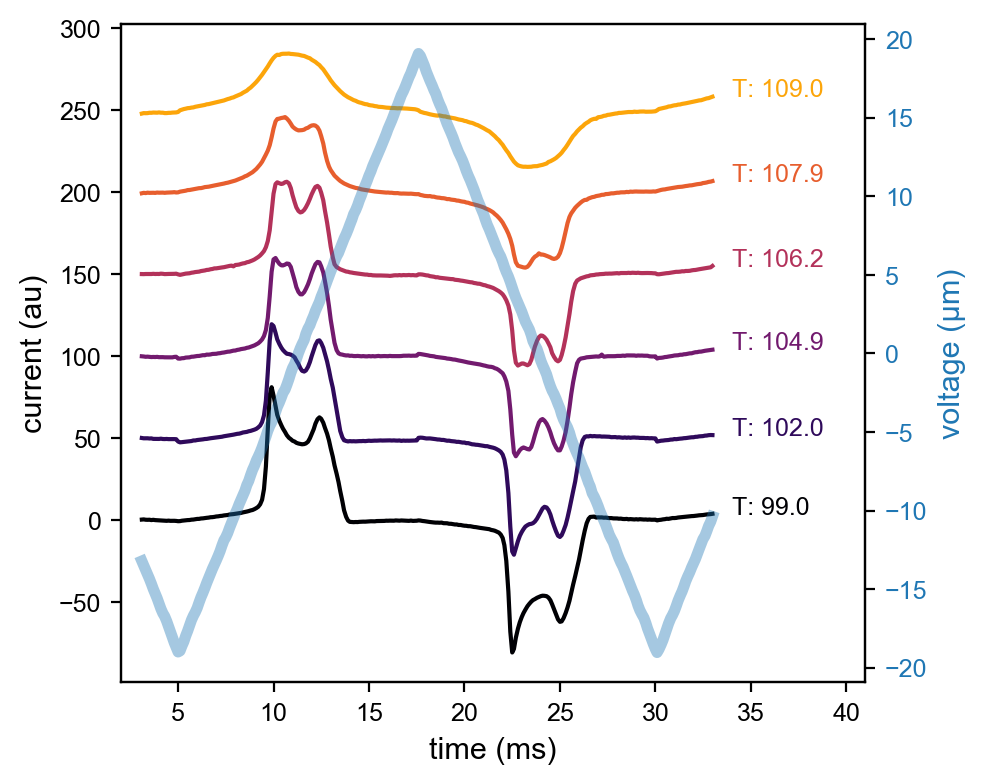
\includegraphics[width=.6\textwidth]{figs/pal30/prc/spacedSm2PRC.png}
%    \caption{\label{fig:pal30:sm2:prc1} Series of polarization current
%        measurements taken in the Sm2 phase of \nfour{}}
%    \end{figure}
%
%A more conventional series of traces for the polarization current is shown in
%\autoref{fig:pal30:sm2:prc1}, where the current is plotted as a function of
%time. The same data is shown in \autoref{fig:pal30:sm2:prc2}, where the
%current is plotted directly against the applied voltage.
%
%\begin{figure}[h!]
%    \centering
%    \includegraphics[width=\textwidth]{figs/pal30/prc/3dplot-sm2.png}
%    \caption{\label{fig:pal30:sm2:prc2} polarization current of sm2 of \nfour{}
%    plotted against applied voltage}
%\end{figure}
%A more conventional series of traces for the polarization current is shown in
%\autoref{fig:pal30:sm2:prc1}, where the current is plotted as a function of
%time. The same data is shown in \autoref{fig:pal30:sm2:prc2}, where the
%current is plotted directly against the applied voltage. The
%
%
%
%\subsection{Freely-Suspended Films of the \smcpalpha{} phase}
%\subsection{X-ray Analysis of the \smcpalpha{} phase}
%
%The two techniques used to characterize the \smcpalpha phase were SAXS (small
%angle hard x-ray scattering) and RSoXS (resonant soft x-ray scattering). As the
%SAXS is sensitive to periodicity in electron density, we can directly measure
%the smectic layer size ($d$), as shown in \autoref{fig:pal30:saxs}. 
%
%\begin{figure}[h!]
%    \centering
%    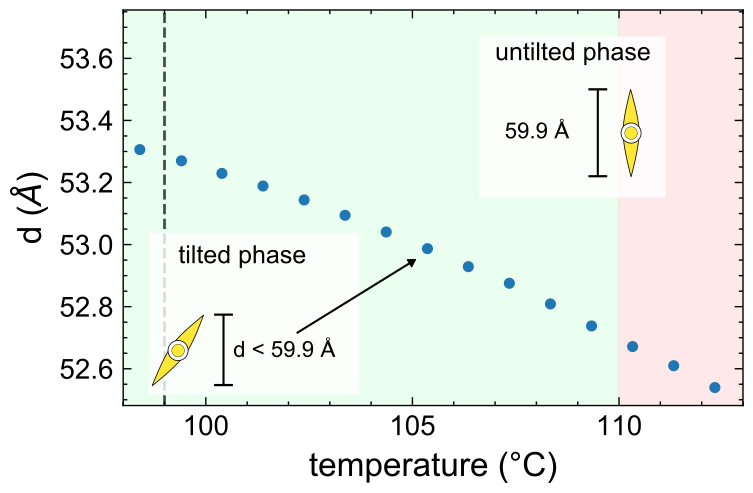
\includegraphics{figs/pal30/xraysm1/sm2-saxs-annote.png}
%    \caption{\label{fig:pal30:saxs} SAXS of \smcpalpha{}. The smectic layer
%    size, $d$, increases monotonically on cooling, with no inflection points
%that would be characteristic of a untilted$\rightarrow$tilted phase transition.}
%\end{figure}
%
%The smectic layer size is measurably smaller than the length of an extended
%molecule, which supports the classification of \smcpalpha{} as a tilted phase.
%However, the increase seen on cooling, which stands in contrast to the
%majority of bent-core materials, may indicate a significant amount of
%intercalation at higher temperatures.  
%
%The x-ray analysis can be greatly supplemented with the addition of resonant
%scattering, which is sensitive to periodicity in orientation. A resonant diffractogram
%taken at \SI{104}{\degreeCelsius} is shown in \autoref{fig:pal30:diffract}.
%
%\begin{figure}[h!]
%    \centering
%    \includegraphics[width=.8\textwidth]{figs/pal30/rsoxssm2/RSoXS-coexistanenceDiffracto.png}
%    \caption{\label{fig:pal30:diffract} Diffractogram of \nfour{} taken in the
%        coexistance region between the \smcpalpha{} ($q\approx
%        \SI{0.04}{\per\angstrom}$) and the \smcapa{} ($q\approx
%    \SI{0.06}{\per\angstrom}$).}
%\end{figure}
%
%By azimuthally averaging diffractograms like the one in
%\autoref{fig:pal30:diffract} and plotting them as a function of temperature,
%\autoref{fig:pal30:diffractVt}, the
%behaviour of the \smcpalpha phase can be determined over its entire temperature
%range.
%
%
%\begin{figure}[h!]
%    \centering
%    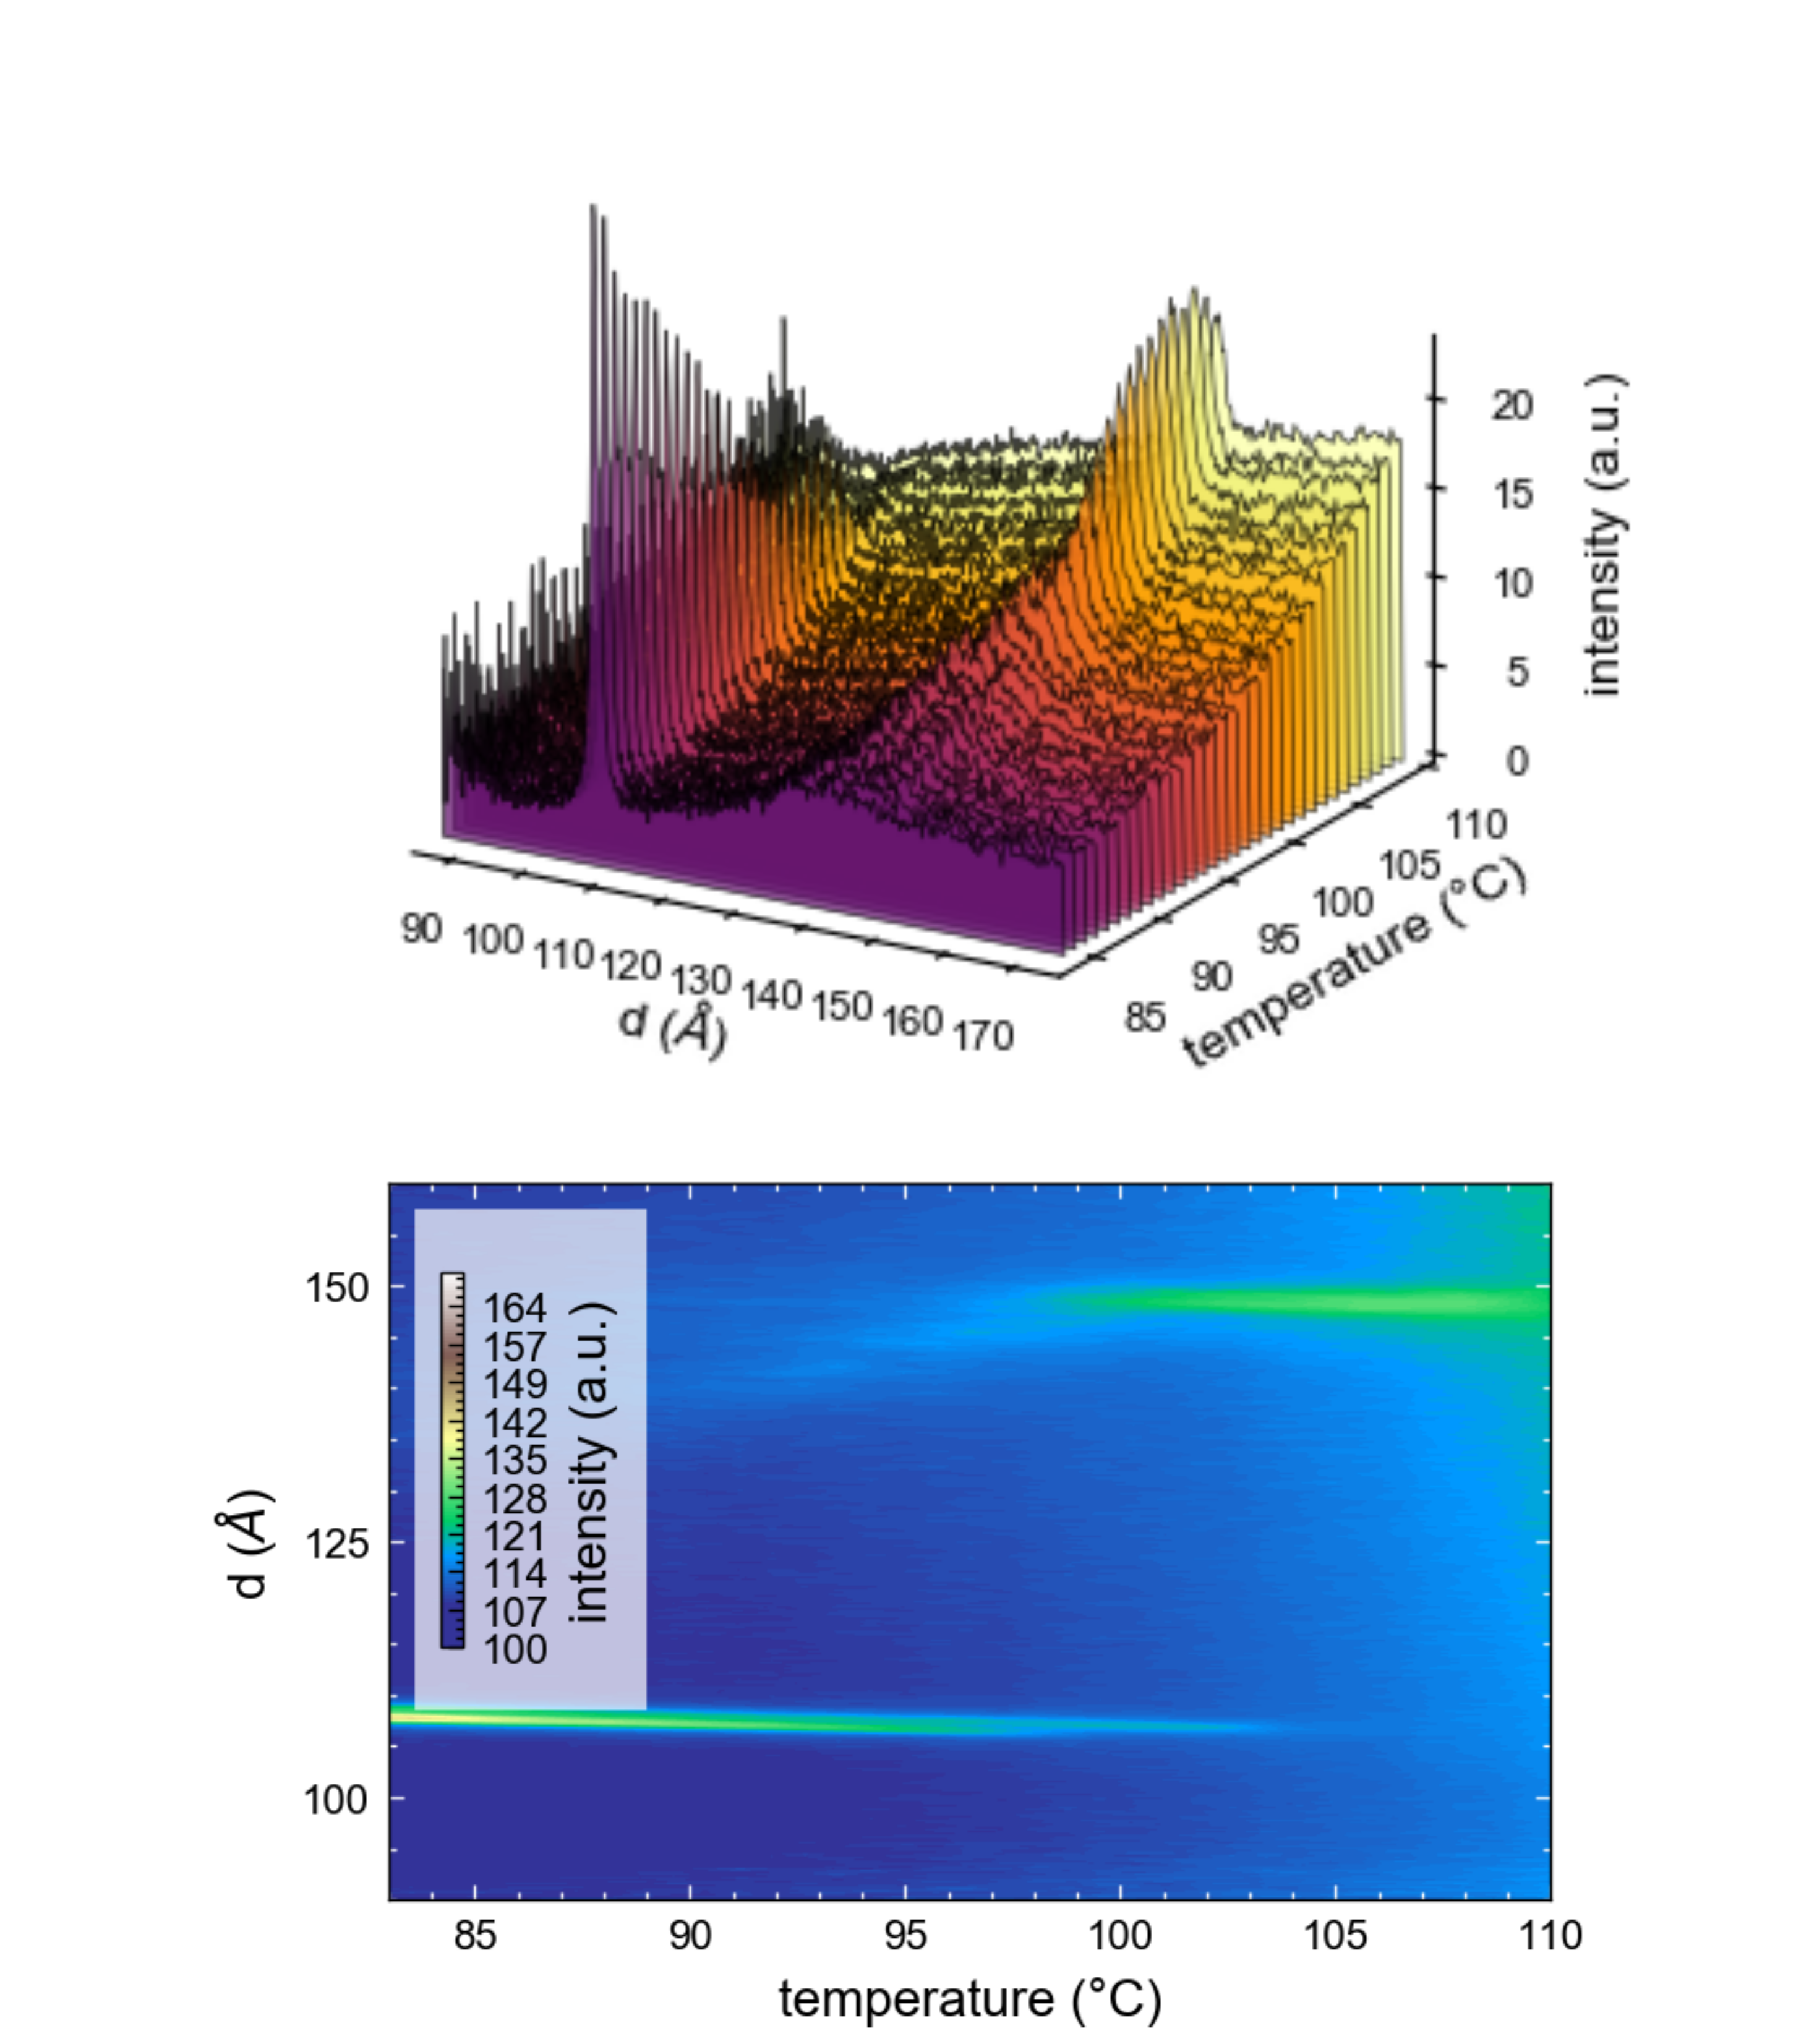
\includegraphics[width=.8\textwidth]{figs/pal30/rsoxssm2/sm2-rsoxs.png}
%    \caption{\label{fig:pal30:diffractVt} Temperature behaviour of the
%    \smcpalpha{} phase plotted as a waterfall plot in (a), and as a contour plot
%    in (b). A bilayer ($d=\SI{112}{\angstrom} =2d_0$) corresponds to the 2-layer
%unit-cell structure of the \smcapa{} phase, which sits directly below the
%\smcpalpha phase in temperature. The resonant peak corresponding to the
%\smcpalpha{} phase at $d\approx\SI{150}{\angstrom}$ is direct evidence that the
%\smcpalpha{} phase is not a classic B2-type phase.}
%\end{figure}
%
%The resonant peak corresponding to the \smcpalpha{} phase
%($d=\approx\SI{150}{\angstrom}$) shows that this phase cannot be a B2 phase (as
%those only have one or two layer unit-cells. However, the fact that this feature
%appears at roughly three times the smectic layer spacing is neccesary but not
%sufficient for a helix. An example of this type of structure would be the
%proposed devil-staircase model put forth to explain a similiar phase in
%\smcstar{} phase family of calimitics.
%
%Though a detailed examination of the unit-cell structure of the \smcpalpha{}
%will have to wait on the advent of polarization-resolved resonant x-ray on the
%carbon K-edge, we can actually confirm the helical nature of the \smcpalpha{}
%phase through careful analysis.
%
%\subsubsection{Umklapp Peaks}
%
%Though a detailed examination of the unit-cell structure of the \smcpalpha{}
%will have to wait on the advent of polarization-resolved resonant x-ray on the
%carbon K-edge, we can actually confirm the helical nature of the \smcpalpha{}
%phase through careful analysis. By combining the SAXS data and the RSoXS data,
%we can deduce two things. First, that the resonant feature of the \smcpalpha{}
%phase is incommensurate with the underlying smectic layer spacing. Specifically,
%it has a unit cell thickness of $\SI{148}{\angstrom}\approx 2.8 d_0$. Second,
%that we are missing an expected umklapp (harmonic) peak.
%
%Umklapp is a german word meaning flip-over, and it refers to higher harmonics
%that are wrapped back into the Brioullon zone. Following Levulet and
%Pansu~\cite{levelut1999tensorial}, where the smectic layers are modeled as
%stacked tensorial slabs, the master equation that predicts these flip-over
%harmonics is given by:
%\begin{equation} \label{eq:levelut}
%\frac{q}{q_0} = 2 \pi l + 2 \pi m\frac{1}{p},\qquad \forall \: l \in \mathbb{N},
%\quad \forall\: m
%\in \mathbb{Z}
%\end{equation}
%where $q$ is the location of the expected harmonic, $q_0$ is the scattering off
%the smectic layer spacing, $p$ is the pitch (in units of the smectic layer
%spacing) of the unit-cell, $l$ is a positive integer, and $m$ is a positive or
%negative integer.
%
%From \autoref{eq:levelut}, we can see one of the nearest harmonics should occur
%at $l=1,m=-1$. For the \smcpalpha{} phase, with a pitch of $p =1/2.8$, we would
%expect to see a harmonic at \todo{include this number}. To highlight this
%analysis, we plot the azimuthally-averaged diffractogram in the co-existence
%region between the \smcpalpha{} and the \smcapa{}, on a $q$-scale
%normalized by the scattering from the smectic layer spacing, $q_0$, in
%\autoref{fig:pal30-xray-combined}.
%
%\begin{figure}[h!]
%    \centering
%    \includegraphics[width=.4\textwidth]{figs/pal30/rsoxssm2/xray-combined.png}
%    \caption{\label{fig:pal30-xray-combined}X-ray scattering from \nfour{phi}.
%            (a) SAXS gives a peak from the smectic layer ordering at $q=q_0$.
%                The RSoXS peak at $q_H$ indicates that there is superlayer
%            orientational ordering with periodicity $d_H$
%                in the Sm2 phase.
%                    In general, superlayer orientational modulation in a smectic
%                generates RSoXS peaks at wavevectors along the layer normal at
%                    $q(l,m) = l(2\pi/d_0) \pm
%                m(2\pi/d_H)$\cite{levelut1999tensorial}.  The
%                    observation of an RSoXS reflection at $q = q(0,1)$ and the
%                absence of an Umklapp peak at $q = q(1,-1)$  in
%                    the Sm2 confirms a superlayer helix with a scattering
%                amplitude
%                    modulation due to the smectic layering that is undetectably
%                weak.
%                    (b) Temperature dependence of resonant scattering. The helix
%                peak at $q_H \approx1/(2.8 d_0)$ becomes diffuse in the Sm3
%            phase. Splitting
%                of the bilayer peak at $q_B$, which would indicate helical
%            precession of the bilayer structure, is not observed.}
%\end{figure}
%
%
%\section{Discussion of the \smcpalpha{} phase}
%
%%\bibliography{pal30}
%\biblio
%%\bibliographystyle{plain}	% or "siam", or "alpha", etc.
%%\bibliography{pal30,refs}		% Bib database in "refs.bib"
%\end{document}
%
%
%
%
%
%
%
%
%
%
%
%
%
%
%
%%outline:
%%[ ] intro: pick up from the intro, remind the reader about bent-core molecules
%%[ ] talk about the homolog series synthesized and summarize previous work
%%[ ] talk about PAL30 characterization
%%[ ] Remaining mysteries of the PAL30 molecule
%%[ ] talk about the other homolog series (additional work needs to be done on
%%these)
%%\section{Introduction and Context}
%%\nfour{phi}, the compound were we discovered bent-core, smectic helicity was orignally
%%investigated by the Dublin group, with an interest towards developing a new
%%bent-core display, based around orthogonal phases. Because a helical, tight-pitch,
%%orthogonal phase will appear dark in homeotropic alignment, but still have a
%%fast field response, it would make for an ideal display. 
%%\begin{figure}[h!]
%%    \centering
%%    \includegraphics[width=.8\textwidth]{./figs/pal30/finalFigs/pal30.pdf}
%%    \caption{Bent-core material \nfour{phi}.}
%%\end{figure}
%%
%%Serving as an excellent example of scientific irony, the Dublin group, though
%%completely correct about the exotic tight-pitch helix of \nfour{phi},
%%mischaracterized the phase as being orthogonal. A cursory look at the
%%planar-aligned textures in Figure~\ref{fig:textures} shows that
%%\nfour{phi} reveals chiral (therefore tilted) phases under application of a
%%field in planar-aligned cells.
%%
%%Because the Dublin's group original analysis was based on: constructing a list
%%of possible orthogonal phases (the \smapf{}, the \smapa{}, the \smap2{}, the
%%\smapalpha{} and the
%%\smapr{} phases); then ruling them out one by one based on the behaviour of
%%the observed \nfour{} phase, the fact that \nfour{} is tilted means that their
%%identification of a tight-pitch phase was right for the wrong reasons.
%%
%%Unfortunately, because \nfour{} is \textit{not} tilted, this removes it from
%%being a potential switching material.
%%- Find original synthesis paper
%%- Talk to Carsten about why they synthesized this phase, so we can include the
%%motivation.
%%- Chirality? (I need to think carefully about chirality, and spontaneous
%%chirality, as this forms a lot of the interesting things about this phase.)
%%- Time for the knives to come out. Discuss their original PRL paper and
%%subsequent MCLC, point out all the reasons for their shitty characterization. We
%%can really go into depth here.
%%
%%\subsection{Characterization}
%%-brief summary of characterization before I joined. (Need to decide how in depth
%%we want to do this i.e. narrative focus, or concise. I'm leaning towards concise
%%actually. This isn't a history lesson, it is a textbook entry on PAL30. 
%%-look at Mike's NTB characterization chapter for inspiration here.
%%\subsection{Modelling}
%%-talk to Matt about this, how does Spartan work?
%%-can he recommend a reference that shows how calculating the smectic layer
%%spacing from this way was actually useful?
%%\subsection{Optical Texture Analysis}
%%The optical textures of planar-aligned (bookshelf) cells of
%%\nfour{phi} were studied using PLM.
%%Upon cooling from the isotropic, the Sm1 phase grows in (at \SI{175}{\degreeCelsius})
%%as b\^{a}tonnets, giving a smooth, focal-conic texture typical of an orthogonal fluid smectic (Figure~\ref{fig:main}(f)).
%%However, given the large value of the estimated
%%molecular tilt, $\theta_\textrm{xray}$, the Sm1 is probably a de Vries
%%smectic.
%%In planar-aligned cells, there is no observable field-induced change of the in-plane birefringence, $\Delta n= n_\parallel
%%-n_\perp$, in small applied electric fields  (Figure~\ref{fig:main}(f)),
%%or in the optic axis orientation, $\theta_\text{opt}$ (Figure~\ref{fig:threshold}).
%%
%%\begin{figure}[h!]
%%    \centering
%%    \includegraphics[width=.8\textwidth]{./figs/pal30/finalFigs/shaoresults-v4.png}
%%    \caption{\label{fig:pal30-texture}Three distinctive optical textures of
%%        \nfour{phi} at zero field (b,e,h) and with a field applied into (a,d,g)
%%        and out of (c,f,i) of the plane of the cell. \nt{still have to fix up
%%    this figure}}
%%\end{figure}
%%
%%
%%Below \SI{115}{\degreeCelsius}, a threshold field, $E_\text{th}$, above which a first-order structural change marked by the appearance of chiral conglomerate domains occurs, becomes experimentally accessible.
%%These domains are polar and exhibit a uniform, saturated optic axis tilt on the
%%order of $\theta_{\rm opt} \approx \SI{18}{\degree}$ from the layer normal, implying that the achiral, untilted Sm1 phase
%%transforms in the field to a B2-like, homochiral \smcspf{phi} state (Figure
%%S1(c))~\cite{eremin2008electrically}. The field-induced left- and right-handed domains form a ``tiger stripe''
%%pattern (Figures~\ref{fig:main}(e,g)). The local domain handedness in this unusual conglomerate texture 
%%is apparently locked in after the first few field cycles.  This bias is due to a chiral
%%memory effect at the surface since, as
%%Figures~\ref{fig:main}(d)~and~\ref{fig:threshold} show, the
%%sub-threshold bulk state has an achiral field response, with a linear polarization current (implying $P \propto E$) and no
%%detectable reorientation of the optical tilt.
%%$E_\text{th}$  decreases strongly on cooling as the transition to the Sm2 phase is approached, as shown in the inset of Figure~\ref{fig:threshold}.
%%%
%%\begin{figure}[h!]
%%    \includegraphics[width=.8\columnwidth]{./figs/pal30/finalFigs/threshold-inset2.png}
%%    \caption{\label{fig:threshold}
%%        Optical tilt of \nfour{phi} vs.\ applied field. The Sm1
%%        phase shows no electrooptic response in weak fields $E<E_\text{th}$. Fields $E>E_\text{th}$ induce an electroclinic
%%        tilt and result in the formation of chiral domains.
%%        $E_\text{th}$, which becomes smaller with decreasing $T$ (inset), matches
%%        closely $E_\text{sat}$, the field at which the induced
%%        polarization saturates, extracted from Figure~\ref{fig:main}(d).
%%        The Sm2 phase exhibits a chiral
%%        electroclinic effect near $E=0$ and hysteresis in the field-induced helix unwinding to the
%%        \smcspf{phi} state.   }
%%
%%\end{figure}
%%
%%
%%In the lower part of the Sm1, and throughout the Sm2, Sm3 and Sm4 phases, the birefringence increases on application of an electric field, as seen in Figure~\ref{fig:main}(c),  changing from yellow to orange.
%%Measurements of $\Delta n$ at $E = 0$ and $E = \SI{20}{\volt\per\micro\metre}$
%%(Figures~\ref{fig:main}(c) and S6),
%%show that the birefringences in the lower temperature
%%phases with and without an applied field are of the order of $\Delta n_\text{on} \sim 0.12$ and $\Delta n_\text{off} \sim 0.10$.
%%Assuming that the field-on \smcspf{phi} state
%%(Figures~\ref{fig:main}(n--p) and S1) gives a uniform
%%director orientation with the optic axis in the plane of the cell, then $\Delta
%%n \sim 0.12$ would correspond to the maximal birefringence $n_3-n_1$ of the
%%\smcspf{phi} state. Modeling the bent-core molecule
%%as two uniaxial, birefringent rods connected with an opening angle of
%%$\Psi$, and tilting this molecule from $z$ by an angle $\theta$,
%%we have calculated the birefringence of all of the states shown in
%%Figure~\ref{fig:main}. If the Sm1 phase is assumed to be a de Vries SmA, with
%%azimuthally averaged molecules distributed on a tilt cone of angle
%%$\theta$, the best fit to the measured birefringence values $\Delta n_\text{on}$ and $\Delta n_\text{off}$ is
%%obtained with $\Psi = \SI{150}{\degree}$ and $\theta = \SI{15}{\degree}$.
%%The calculated birefringence as a function of temperature is shown in Figure~S6.
%%
%%
%%
%%The transitions between the smectic phases are difficult to see when $E=0$ because they are all orthogonal in appearance,
%%with an optic axis along $z$, and have similar birefringence.
%%At the transition from Sm1 to the Sm2 phase,  however, arbitrarily small electric fields induce molecular tilt in the
%%(Figure~\ref{fig:threshold}), leading to the formation of optically distinct, conglomerate chiral
%%domains with opposite tilt (Figures~\ref{fig:main}(h--j)), again
%%corresponding to a field-induced transition to a \smcspf{phi} state.
%%The birefringence and orthogonal appearance of the Sm2 ground state are consistent with
%%the helical superlayer structure indicated by RSoXS.
%%
%%The texture and birefringence of the Sm3 phase in the absence of field are consistent with the \smcapa{phi} bilayer structure indicated by RSoXS.
%%The field-induced conglomerate domain morphology in both the Sm2 and Sm3 phases is distinct from that of the undulating Sm1
%%tiger stripes, with straight
%%domain boundaries that tend to form parallel to the layers, as in an
%%antiferroelectric calamitic being driven to a ferroelectric
%%state~\cite{li1995reversible}.
%%The optical tilt in these domains is found to be $\theta_\mathrm{opt}\sim 18^\circ$.
%%
%%The response to applied field changes dramatically again at
%%the transition from Sm3 to Sm4, with no visible brush rotation or evidence of domain formation at any $E$. The birefringence in the Sm4 phase increases continuously with field, saturating
%%at a value comparable to that observed in the field-induced Sm2 and Sm3 conglomerate domains.
%%
%%\nfour{phi} transitions into a SmA-like phase from the isotropic phase at
%%\SI{174}{\degreeCelsius}. This phase is optically confirmed to be smectic as
%%the smectic layer undulations give rise to characteristic stripes parallel
%%to the layer normal. These smectic domains grow in as batonnets \nt{fix accent},
%% which is again, characteristic to SmA phases. Further cooling results in
%% the development of ``tiger stripe'' textures on application of high fields
%% (fields larger than some temperature dependent threshold voltage).
%%
%% These ``tiger stripe'' textures are unique to the \nfour{phi} molecule, and
%% are characterized by wavy undulations of alternating bright and dark
%% regions that form parallel to the smectic layers. Though the specific
%% dynamics that set the size of these tiger stripes is currently unknown,
%% they are thought to form during a transition to chirality, that will be
%% discussed in more detail.
%%
%%
%%\subsection{Polarization Reversal Current}
%%\begin{figure}[h!]
%%    \centering
%%    \includegraphics[width=.8\textwidth]{./figs/pal30/finalFigs/polzv9.png}
%%    \caption{\label{fig:pal30-prc}Polarization-reversal current of \nfour{phi}.
%%            A \SI{40}{\hertz} triangular voltage  
%%                with an amplitude of \SI{72}{\volt} was applied to \nfour{phi} 
%%                    in a \SI{4.5}{\micro\metre} Instec cell. The voltage
%%                    zero-crossing
%%                        is at $t=0$. Three
%%                            (ferrielectric) current peaks are visible from
%%                                approximately \SIrange{110}{99}{\degreeCelsius},
%%                                two
%%                                    (antiferroelectric) peaks from
%%                                    \SIrange{99}{83}{\degreeCelsius}, and a
%%                                        single (ferroelectric) peak from
%%                                        \SIrange{83}{60}{\degreeCelsius}.
%%                                            The corresponding liquid crystal
%%                                            phases are indicated schematically
%%                                            using
%%                                            the same color scheme as in Figure
%%                                            1. Three polarization switching
%%                                            peaks are understood to
%%                                            be associated with helical unwinding
%%                                            (see the discussion of the
%%                                            SmC$^{*}_\textrm{FI1}$ calamitic
%%                                            phase in Takazoe et
%%                                            al.~\cite{takezoe2010antiferroelectric}),
%%                                            in contrast with the
%%                                            SmC$^{*}_\alpha$ calamitic phase,
%%                                            which displays
%%                                            antiferroelectric (two peak)
%%                                            behaviour~\cite{lagerwall2005demonstration}.
%%                                            Though we believe the Sm2 is best
%%                                            described as an incommensurate
%%                                            Sm(CP)$_\alpha$ phase, the pitch
%%                                            ($\approx 2.8$-layer) is much closer
%%                                            to the $3$-layer
%%                                            pitch of the SmC$^{*}_\textrm{FI1}$
%%                                            than the Sm$^{*}_\alpha$ calamitic
%%                                            phases
%%                                            (typically 5--50 layers),
%%                                            which may explain why we see
%%                                        ferrielectricity.} 
%%\end{figure}
%%The polarization reversal current, measured with a triangular
%%applied field, is shown vs.\ temperature in Figures~\ref{fig:main}(d) and
%%S7. Upon cooling from the isotropic, a single current bump centered
%%about $E=0$ first appears at lower temperatures in the Sm1 phase, indicating a Langevin-type
%%field-induced orientation of $\mathbf{P}$, with a linear response near $E=0$
%%and the current vanishing  when $\mathbf{P}$ becomes saturated (for $E \ge E_\text{sat}$).
%%Significantly, $E_\text{sat}$ is similar in magnitude to $E_\text{th}$, the threshold
%%field required for the Sm1
%%transition to chirality observed optically (Figure~\ref{fig:threshold}, inset), indicating that the
%%field first orders the Langevin system of initially azimuthally random molecular
%%polarizations, with the Sm1 remaining in an achiral state, and that the phase becomes
%%chiral only at higher fields, once $\mathbf{P}$ is saturated (Figure S8). Upon entering the
%%Sm2, this polarization bump splits into three peaks roughly centered about
%%$E=0$, coalescing into two peaks on cooling through the Sm3.
%%\nfour{phi} thus transforms on cooling from the non-polar
%%Langevin ground state of the Sm1, where $P=0$ is enforced by entropy, to energetically stabilized ground
%%states in which the spatial average of
%%$\mathbf{P}(\mathbf{r})$ in the absence of applied field is also zero: the incommensurate helical winding of the
%%polarization
%%in the Sm2, and the antiferroelectric bilayer structure in the Sm3. At the
%%transition to the Sm4, a single, broad current peak reappears, characteristic of the block
%%polarization switching of a ferroelectric ground state that is surface-stabilized
%%with $\mathbf{P}$ parallel to the cell plates at $E=0$, such as occurs in the orthorhombic \smapf{phi} phase~\cite{shen2011effective}.
%%The absence of brush rotation during the field-induced reorientation of the
%%polarization in Sm4 is consistent with achiral \smcapf{phi} superlayer organization.
%%
%%\subsection{X-Ray Scattering}
%%-- another figure highlighting the tiger stripes
%%Undoubtably, the most powerful probe in revealing the nanoscale structure of
%%these phases of matter is light, specifically, light small enough to resolve
%%this nanoscale structure: X-rays. (digression on Rayleigh resolution/scattering theory?)
%%
%%For the characterization of PAL30, we used both Small Angle X-ray Scattering
%%(SAXS) and Resonant Soft X-ray Scattering (RSoXS). For the SAXS, we used the
%%Synctron Source at ZZ, confirming these diffractograms with a ZZ (in house)
%%source, shown in Figure XX. 
%%
%%
%%\nt{include multifig with all the traces on it}
%%
%%\begin{figure}[h!]
%%    \centering
%%    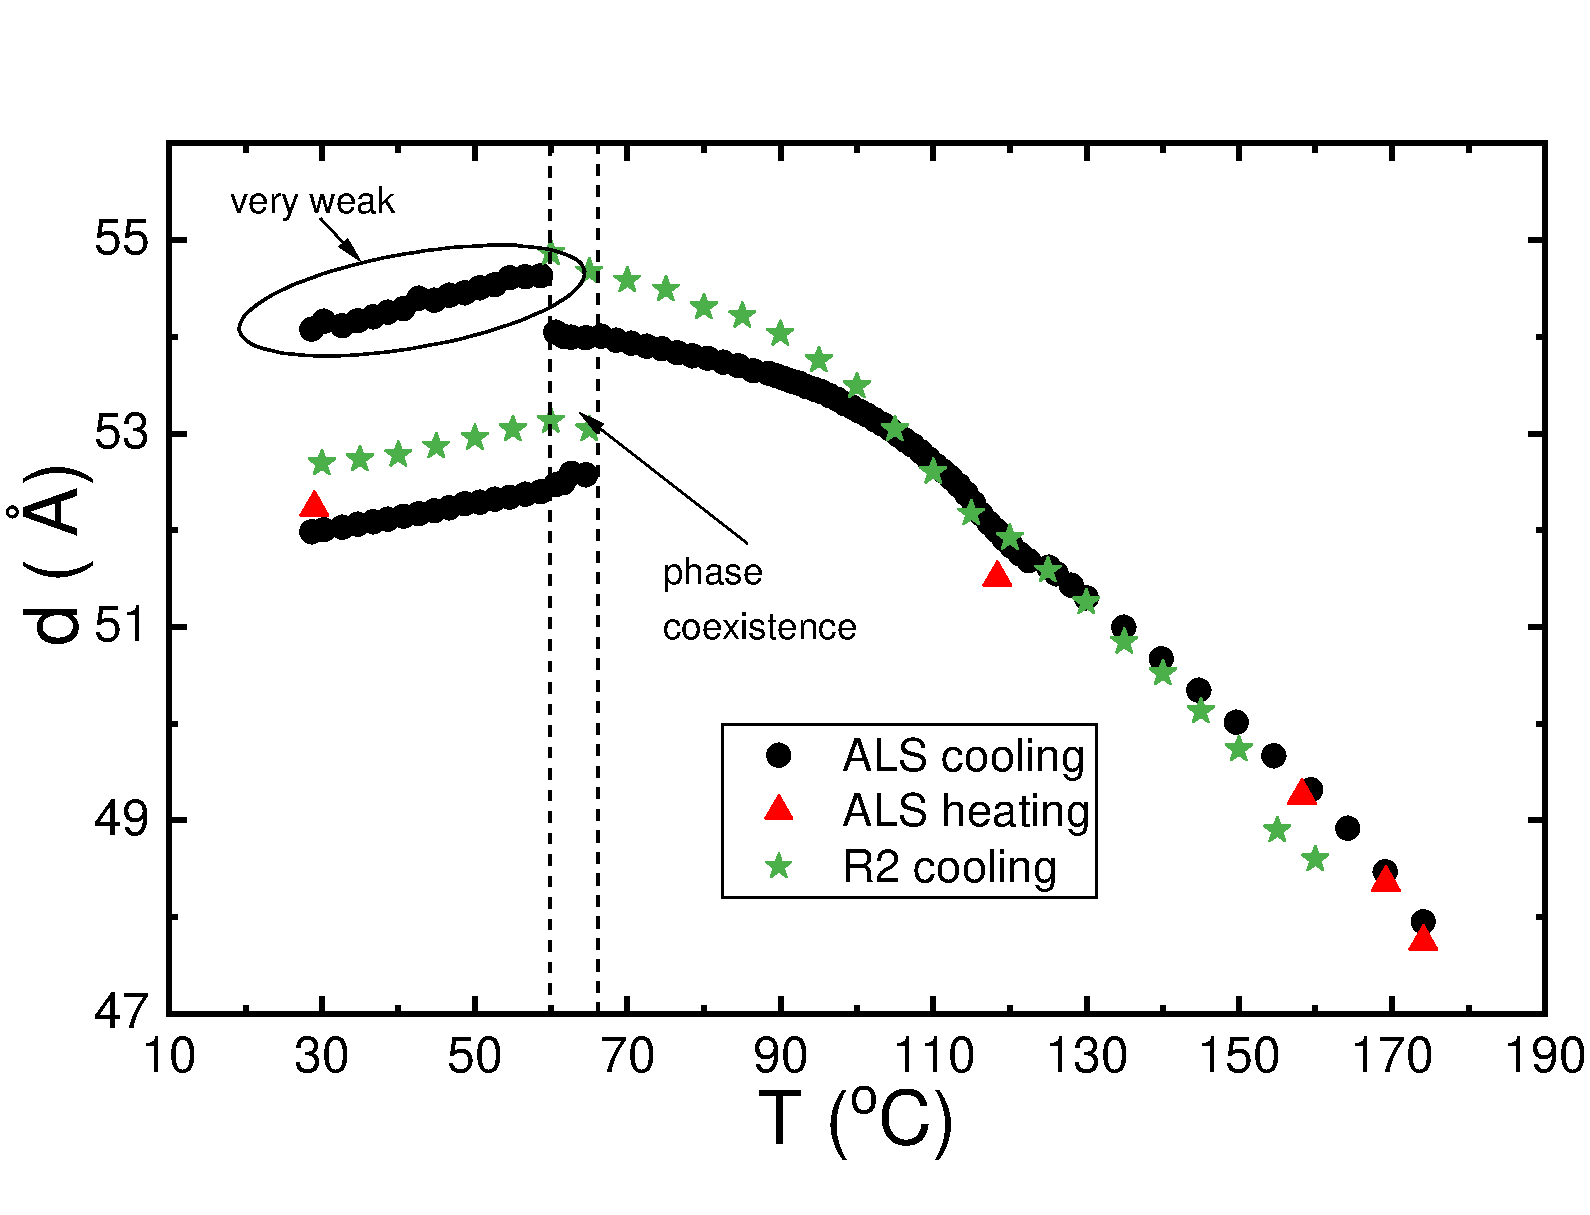
\includegraphics[width=.8\textwidth]{./figs/pal30/finalFigs/combinedALSandR2andAlex.pdf}
%%    \caption{test}
%%\end{figure}
%%As SAXS reveals the underlying electron density structure, it is a powerful,
%%though oftentimes, blunt tool for revealing the phase structure. For PAL30, we
%%observed only a single Bragg peak at $\approx \SI{50}{\angstrom}$. The absence
%%of harmonic peaks indicate that the underlying electron density is very close to
%%being perfectly sinusoidal, allowing for decomposition into a singular Fourier
%%wavelength which corresponds to the smectic layer spacing.
%%
%%%[ ] look at scattering of 8cb (I think Noel mentioned that this was also very
%%%[ ] What does the height of the peak tell you? Look at old scattering theory
%%%books (ashcroft)
%%
%%
%%
%%-include all the SAXS figures, (can we replot them onto the same graph?)
%%- Discuss smectic layer spacing, talk about what else we can determine from this
%%-include RSOXS figures (main one).
%%- orientational at approx $2.8 d_0$, talk about what this could be? Chew the fat
%%on this one.
%%\subsection{Resonant Soft X-ray Scattering}
%%Resonant soft X-ray scattering (RSoXS), as discussed in
%%Section~\ref{sec:int-rsoxs}, is sensitive to periodicities in the orientation of
%%the underlying molecules. The RSoXS scans for PAL30 were carried out by Dr.
%%Michael Tuchband at the Synctron Source in Berkeley.
%%\nt{include relevant preamble from the supplement about the Berekely facilities}
%%X-ray scattering from \nfour{phi} is shown in Figures~\ref{fig:main}(b) and S3.
%%Upon  cooling from the isotropic, a single, non-resonant SAXS peak
%%appears at $\SI{175}{\degreeCelsius}$, at a wavevector $q_0$  corresponding to Bragg scattering from
%%the smectic layers in the Sm1 phase with spacing $d_0 = 2\pi/q_0
%%= \SI{48}{\angstrom}$. The layer spacing increases slightly on cooling
%%to the crystal phase at \SI{65}{\degreeCelsius} and is
%%consistently smaller than the calculated molecular length, $l = \SI{59.9}{\angstrom}$, throughout this temperature range, suggesting that the molecules are tilted in all of the smectic phases, to first order by an average amount estimated using $\theta_\textrm{xray} =
%%\cos(d_0/l)$ of $\SI{33}{\degree}$ (see Figure~S4).
%%In the Sm1 temperature range ($\SI{110}{\degreeCelsius} \leq T \leq
%%\SI{175}{\degreeCelsius}$), there are no RSoXS scattering features that would indicate a
%%superlayer periodic structure (see Figure~S2 and the Supplemental video).
%%
%%At the transition to the Sm2 phase, at $\SI{110}{\degreeCelsius}$, marked  by
%%a distinct enthalpy peak in the DSC (Figure~S5
%%), a single, sharp
%%resonant peak appears at $q_H = \SI[per-mode=reciprocal]{.042}{\per\angstrom}$, corresponding
%%to a molecular orientational structure with a period
%%$d_H=\SI{148}{\angstrom}\approx 2.8 d_0$ that is incommensurate with the
%%smectic layer spacing (Figure~\ref{fig:xray-results}(b)). Below
%%$\SI{104}{\degreeCelsius}$, this reflection
%%becomes weaker and another sharp, resonant reflection at higher $q$ grows in, the coexistence
%%indicating a first-order transition to the Sm3 phase.
%%This second Bragg peak, which persists down to the crystal phase, has a
%%wavevector $q_B\approx q_0/2$, indicative of a commensurate, bilayer orientational
%%structure in the Sm3 and Sm4 phases.
%%%
%%Below \SI{99}{\degreeCelsius}, the incommensurate peak broadens dramatically and
%%moves to higher $q$, indicating the presence of short-ranged, Sm2-like helical
%%fluctuations persisting in the Sm3 phase, and disappears at the transition to the Sm4
%%phase at \SI{83}{\degreeCelsius}. The Sm4 phase exhibits only the bilayer RSoXS
%%reflection at $q_B$.
%%
%%\begin{figure}[h!]
%%    \centering
%%    \includegraphics[width=.8\columnwidth]{./figs/pal30/finalFigs/xray-combined.png}
%%    \caption{\label{fig:xray-results}X-ray scattering from \nfour{phi}.
%%        (a) SAXS gives a peak from the smectic layer ordering at $q=q_0$.
%%        The RSoXS peak at $q_H$ indicates that there is superlayer orientational ordering with periodicity $d_H$
%%        in the Sm2 phase.
%%        In general, superlayer orientational modulation in a smectic generates RSoXS peaks at wavevectors along the layer normal at
%%        $q(l,m) = l(2\pi/d_0) \pm m(2\pi/d_H)$\cite{levelut1999tensorial}.  The
%%        observation of an RSoXS reflection at $q = q(0,1)$ and the absence of an Umklapp peak at $q = q(1,-1)$  in
%%        the Sm2 confirms a superlayer helix with a scattering amplitude
%%        modulation due to the smectic layering that is undetectably weak.
%%        (b) Temperature dependence of resonant scattering. The helix peak at $q_H \approx1/(2.8 d_0)$ becomes diffuse in the Sm3 phase. Splitting
%%        of the bilayer peak at $q_B$, which would indicate helical precession of the bilayer structure, is not observed.
%%        }
%%\end{figure}
%%
%%
%%The RSoXS scattering from a single layer can be analyzed, following Levelut and
%%Pansu, in terms of a monoclinic second-rank tensor with a principal
%%axis tilted from and then azimuthally rotated about the layer normal~\cite{levelut1999tensorial,gleeson_resonant_2006,Barois2012review}.   Scattering
%%from a stack of such layers is calculated by summing over the contributions of the individual layers at different $z$.
%%Resonant scattering peaks from azimuthally
%%periodic arrangements are found at wavevectors along $z$, $q(l,m) = l(2\pi/d_0)
%%\pm m(2\pi/p)$, where $p$ is the pitch.  In principle, resonant
%%scattering should appear at all values of $l$ (harmonics of $q_0$), and at values
%%of $m=0,\pm1,\pm2$ that depend on the superlayer structure.  In an incommensurate, helical
%%structure, like the SmC$_\alpha$ phase, only the fundamental and harmonic peaks at
%%$q(l=0,m=+1,+2)$ and the Umklapp peaks at
%%$q(l=+1,m=-1,-2)$ are found in the range $0 < q(l,m) <
%%q_0$. If the resonant scatterers are confined to lie precisely on layers spaced
%%by $d_0$, then the intensities of these peaks will be identical~\cite{levelut1999tensorial}.
%%Out-of-layer molecular positional fluctuations, and, in particular,
%%those for which there is a coupled azimuthal orientation that keeps the molecule
%%on the helix, $\delta \phi = (2\pi/p)\delta z$, reduce the intensities of the
%%resonant harmonic peak
%%at $2q_H$ and of the Umklapp peaks at $q_0 \pm q_H$, relative to that of the fundamental at
%%$q_H$~\cite{levelut1999tensorial}. In our RSoXS scans of these peaks, only the
%%fundamental is seen above the background, so that only the upper limit of
%%the intensity ratio of the Umklapp and fundamental peaks
%%can be estimated. From the RSoXS heating scan of
%%Figure~\ref{fig:xray-results}(a), we find $I_\text{U}/I_\text{F} \lesssim 0.03$, implying a very
%%weak fractional modulation of the density of helical scatterers, $\rho$, due to fluctuations in the
%%smectic layering $\sqrt{\langle\delta\rho^2\rangle}/\rho_0 < 0.17$. The absence of the harmonic peaks places a similar limit on how much the density modulation of helical scatterers deviates from being purely sinusoidal.
%%
%%\begin{figure}[h!]
%%    \centering
%%    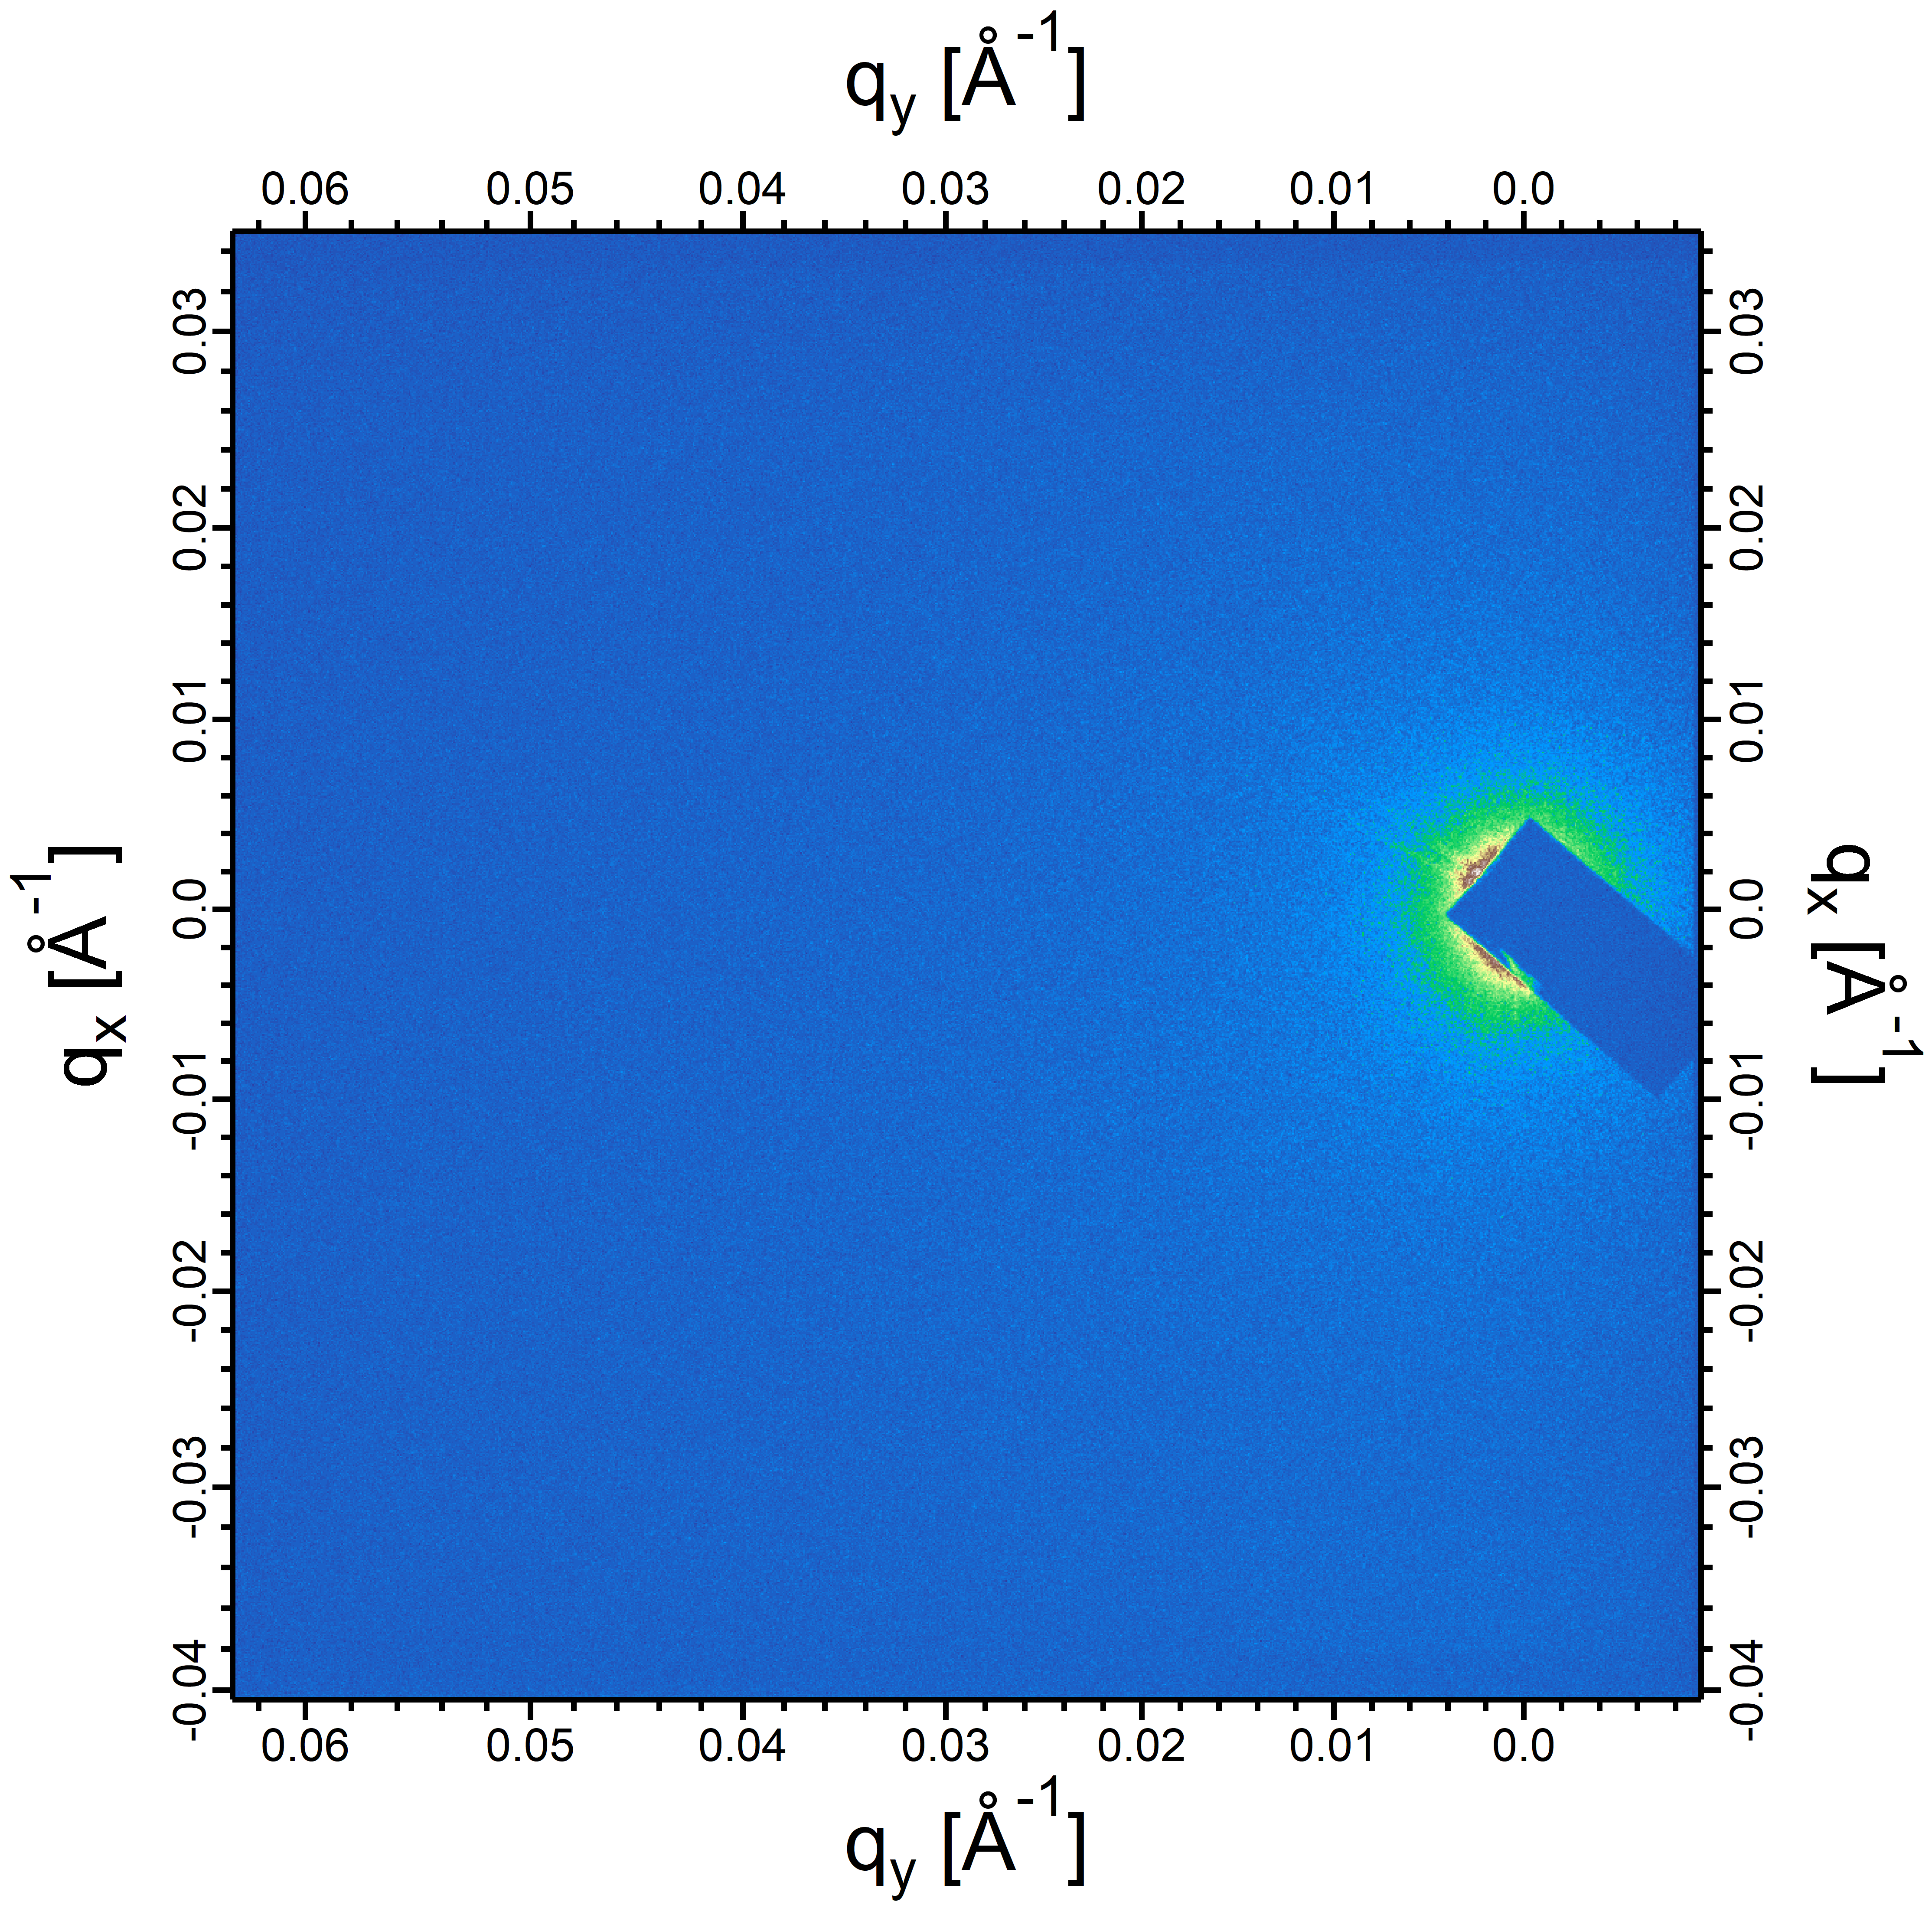
\includegraphics[width=.8\textwidth]{./figs/pal30/finalFigs/rsosxSmaT113-modified.png}
%%	\caption{\label{fig:rsoxs-sm1} Resonant soft X-ray scattering (RSoXS) of \nfour{phi} observed in
%%        the Sm1 phase ($T=\SI{113}{\degreeCelsius}$). This image is
%%        characterisitic of the phase. The absence of any
%%        resonant scattering features is characteristic of the Sm1 showing that
%%        there are no periodic
%%    structures present.}
%%\end{figure}
%%
%%\begin{figure}[h!]
%%    \centering
%%    \includegraphics[width=.8\textwidth]{./figs/pal30/finalFigs/RSoXS-coexistanenceDiffracto.png}
%%    \caption{\label{fig:rsoxs-coexistDiff} Diffractogram from PAL30 cooling run
%%        carried out at the Berekely facilities in the coexistance region between
%%        Sm1 and Sm2. Periodic features are seen at $q\approx
%%    \SI[per-mode=reciprocal]{.004}{\per\angstrom}$ and $q\approx
%%\SI[per-mode=reciprocal]{.006}{\per\angstrom}$.}
%%\end{figure}
%%
%%These features were confirmed to be resonant peaks by scanning the beam-line
%%energy through a range, as shown in Figure~\ref{fig:resonant-energy-scan}.
%%\begin{figure}[h!]
%%    \centering
%%    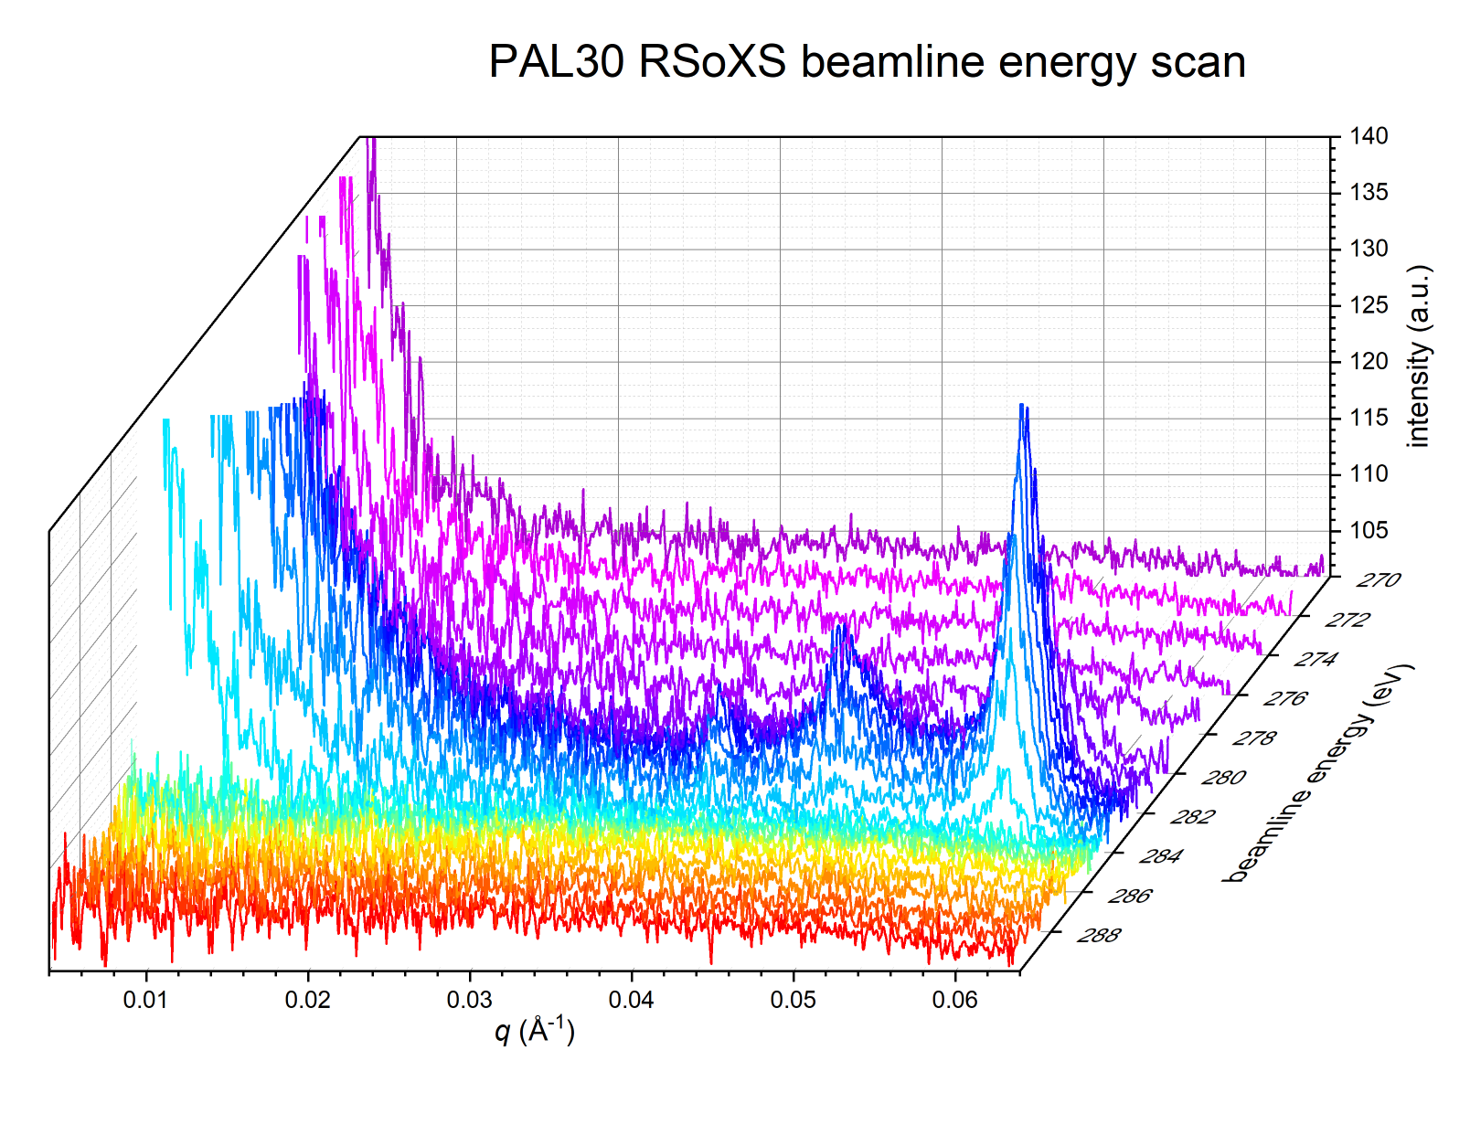
\includegraphics[width=.8\textwidth]{./figs/pal30/finalFigs/resonsnat-energy-scan.png}
%%    \caption{\label{fig:resonant-energy-scan} The peaks seen at
%%        \SI{102}{\degreeCelsius} in Figure~\ref{fig:rsoxs-coexistDiff} disappear
%%        as the beam-line energy is scanned through a range of values, confirming
%%        that they are resonant, i.e./ they correspond to periodicities in
%%    \textit{orientation} not \textit{density}.}
%%\end{figure}
%%
%%\begin{figure}[h!]
%%    \centering
%%    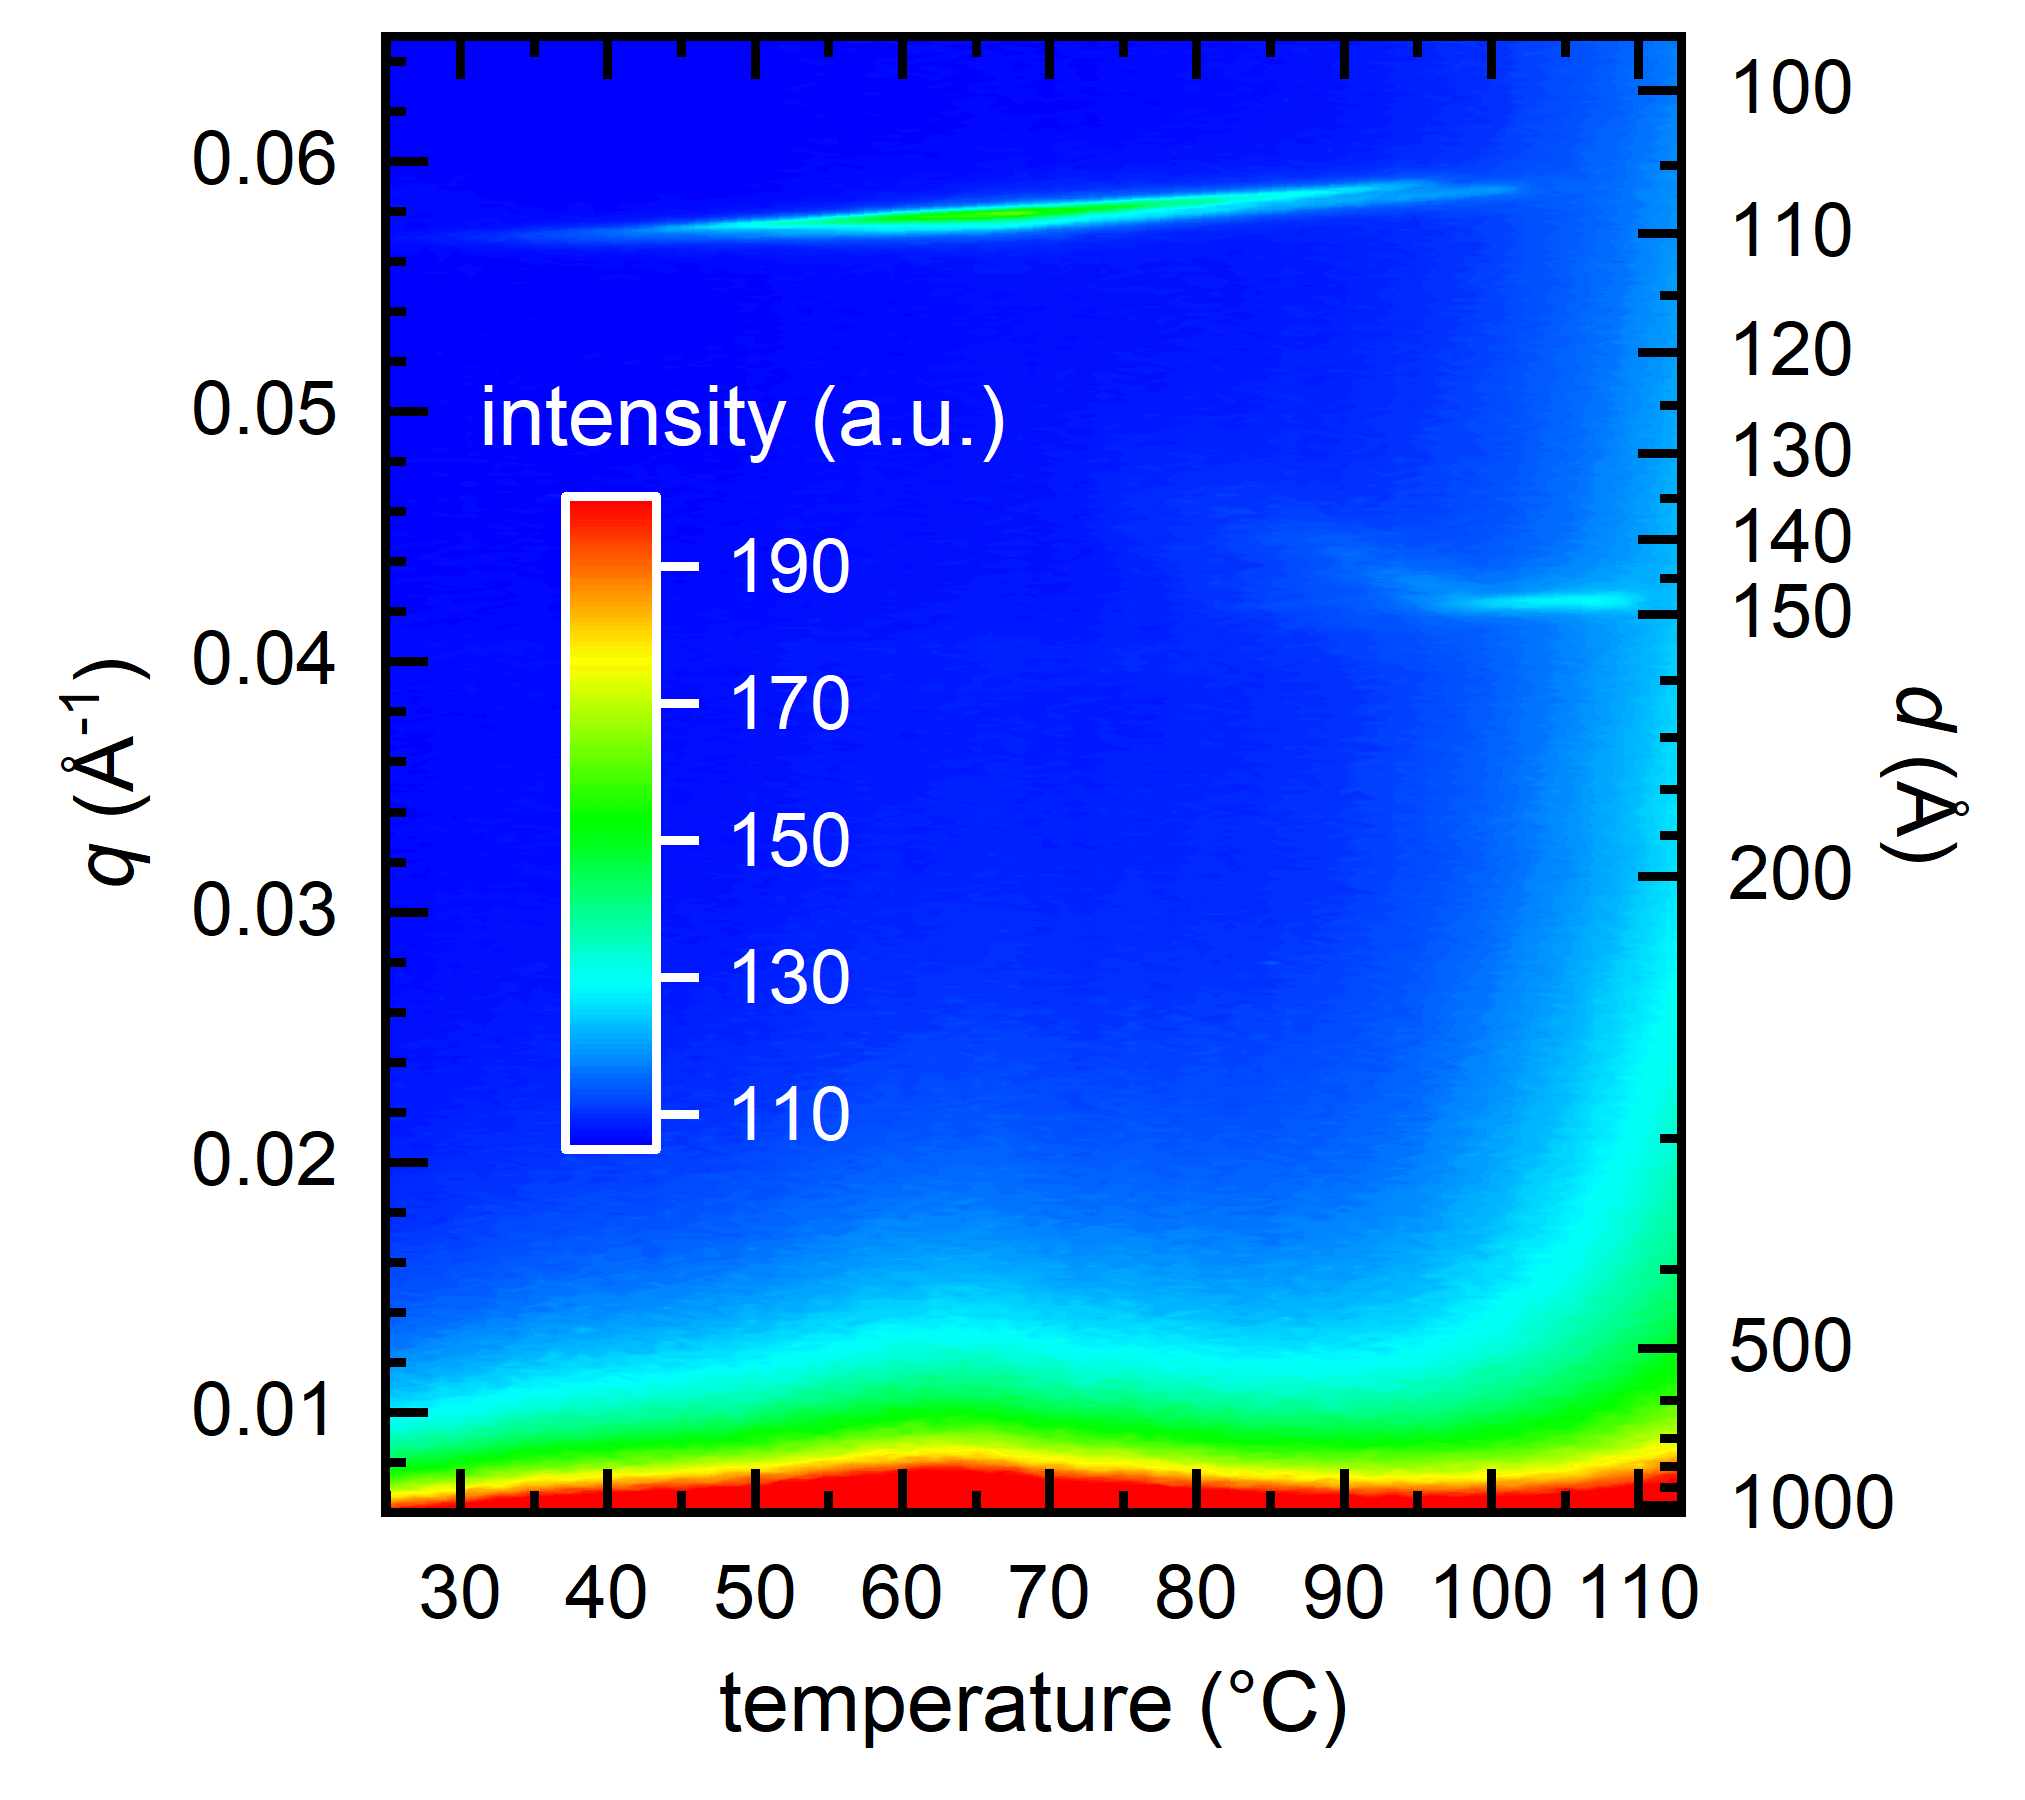
\includegraphics[width=.8\textwidth]{./figs/pal30/finalFigs/PAL30RSOXSshiftedTcontourplotv1mt.png}
%%    \caption{\label{fig:rsoxs-main} Resonant soft X-ray scattering (RSoXS) of \nfour{phi} observed
%%        vs.\ temperature on
%%    cooling. The plot was generated
%%    from a temperature series of 2D diffractograms that were azimuthally
%%    averaged, then interpolated and plotted in $q$-space with corresponding real-space coordinates
%%    ($d=2\pi/q$). Above \SI{110}{\degreeCelsius}, we
%%    observe no scattering features, indicating the absence of resonant structures periodic in
%%    this $d$-range. On cooling below \SI{110}{\degreeCelsius}, a scattering arc
%%    appears at $d=\SI{148}{\angstrom}$, corresponding to  about three smectic layer
%%    spacings.
%%    This reflection persists on further cooling but becomes weaker and
%%    disappears
%%    at \SI{99}{\degreeCelsius}. At
%%    \SI{105}{\degreeCelsius}, a second feature appears (at $d =
%%    \SI{107}{\angstrom}$)
%%    corresponding to two smectic layer spacings. This feature
%%    shifts to smaller $q$, and then disappears at the transition to the
%%    crystal phase at \SI{65}{\degreeCelsius}. In the $q$ range we investigated
%%    (corresponding to \SIrange{50}{1256}{\angstrom}), we see no other orientational modulations.}
%%\end{figure}
%%
%%\begin{figure}[h!]
%%    \centering
%%    \includegraphics[width=.8\textwidth]{./figs/pal30/finalFigs/xray-combined.png}
%%    \caption{\label{fig:xray-combined} X-ray scattering from \nfour{phi}.
%%        (a) SAXS gives a peak from the smectic layer ordering at $q=q_0$.
%%        The RSoXS peak at $q_H$ indicates that there is superlayer orientational ordering with periodicity $d_H$
%%        in the Sm2 phase.
%%        In general, superlayer orientational modulation in a smectic generates RSoXS peaks at wavevectors along the layer normal at
%%        $q(l,m) = l(2\pi/d_0) \pm m(2\pi/d_H)$\cite{levelut1999tensorial}.  The
%%        observation of an RSoXS reflection at $q = q(0,1)$ and the absence of an Umklapp peak at $q = q(1,-1)$  in
%%        the Sm2 confirms a superlayer helix with a scattering amplitude
%%        modulation due to the smectic layering that is undetectably weak.
%%        (b) Temperature dependence of resonant scattering. The helix peak at $q_H \approx1/(2.8 d_0)$ becomes diffuse in the Sm3 phase. Splitting
%%        of the bilayer peak at $q_B$, which would indicate helical precession of the bilayer structure, is not observed.
%%        }
%%    \end{figure}
%%
%%    \nt{discussion of what this all means, with theory digression to explain the
%%    flucuations}
%%\subsection{Comparison to Previous Phases}
%%\subsection{Remaining Mysteries and Inconsistancies}
%%-Look at list that I've written down here. (Should work on this firstish, so we
%%can send it to Leo.)
%%\section{Homologous Series of PAL30}
%%
%%\end{document}
